\documentclass[10pt,a4paper]{article}
\usepackage[hmargin=1.5cm,vmargin=1.5cm]{geometry}
\usepackage{fancyhdr}
\usepackage{tabulary}
\usepackage{graphicx}
\usepackage{amssymb}
\graphicspath{{./latex_images/}}
\begin{document}
\pagestyle{fancy}
\fancyhead[L]{0801CS211051}
\fancyhead[R]{Kartik Baghel}
\fancyfoot{}
\fancyfoot[R]{\thepage}
\begin{flushleft}
AIM :- To show how a vending machine works\\
\bigskip
\begin{center}
Functions
\end{center}
Function 1 :- Welcome\\
It welcomes the user to vending machine.\\ 
\bigskip
Function 2 :- Rules\\
It tell the use what not to do to vending machine.\\
It tell that the user can buy a single type of product at a time.\\
\bigskip
Function 3 :- Snacks\\
This function is called when the user press 1 for choosing snacks.In this function it prints the name of the snacks available in the vending machine with the price and weight of the snack and a special code is given to every variety of snack. After printing the available snacks it calls selction\_snack function and it stores its value in a variable called amount.\\
\bigskip
Function 4 :- Selection\_snack\\
In this function it first ask the code and quantity of the desired product and after that if else condition is runned on the basis of code entered. If the code entered is matched with the product code it tells the total price of the product and if the code is not matched with any of the if condition else condition is runned and in it a goto statement is used with directly takes the user to the line where the user was asked to enter the code of the product.
After the matching of the code with if condition it calculates the total price of the product by multiplying the quantity of the product to price of the product.This Function giver total\_amount as the return value.This value is stored on the variable amount in snack function.\\
\bigskip
Function 5:- Drinks\\
If the user press 2 in the selection option.He will be directed to drinks function.In this function all the available drinks in vending machine is displayed to the user.Every drink is given a special code.Price and volume of the drink is also displayed.After the displayed of the information of the drinks selection\_drinks function is called and its value is stored in variable amount.\\
\bigskip
Function 6:- Selection\_drinks\\
In this function it first ask the code and quantity of the desired product and after that if else condition is runned on the basis of code entered. If the code entered is matched with the product code it tells the total price of the product and if the code is not matched with any of the if condition else condition is runned and in it a goto statement is used with directly takes the user to the line where the user was asked to enter the code of the product.
After the matching of the code with if condition it calculates the total price of the product by multiplying the quantity of the product to price of the product.This Function giver total\_amount as the return value.This value is stored on the variable amount in drink function.\\
\bigskip
Function 7 :- Deposit\\
This function basically takes money deposit from the user. it returns the money in the main function from where it was called and the returned amount is store in the variable named as cash.\\
\bigskip
Function 8 :- Cashback\\
It take one integer type datatype as a parameter which is cash.This function basically calculates that your entered amount is is sufficient or not if it is not sufficient shortage\_deposit is called and its value is stored in the valuable remaining,This function gives remaining*-1 as return value.\\
\bigskip
Function 9:- Shortage\_deposit\\
this function basically tells the user that you are short on \_\_\_ amount of money and then ask user to input more money. Even after giving more money if its lesser then the amount shortage\_deposit function is called again like in recursion and if the total cash is larger then the amount of product then remaining is given as returned value.\\
\bigskip
Function 10:- Again \\
This function ask the user to press 1 if user want to buy something else and press 2 to quit. If the user presses 1 then shop\_again function is called and if the user press 2 then thanks message is printed and on entering any other value it will print you pressed wrong number and a goto statement will take you to give the response again.\\
\bigskip
Function 11:- Shop\_again\\
this function basically calls all the required function in a sequential way. It does not print the welcome and rules message. 
\newpage
\begin{center}
Profiling Report\\
\bigskip
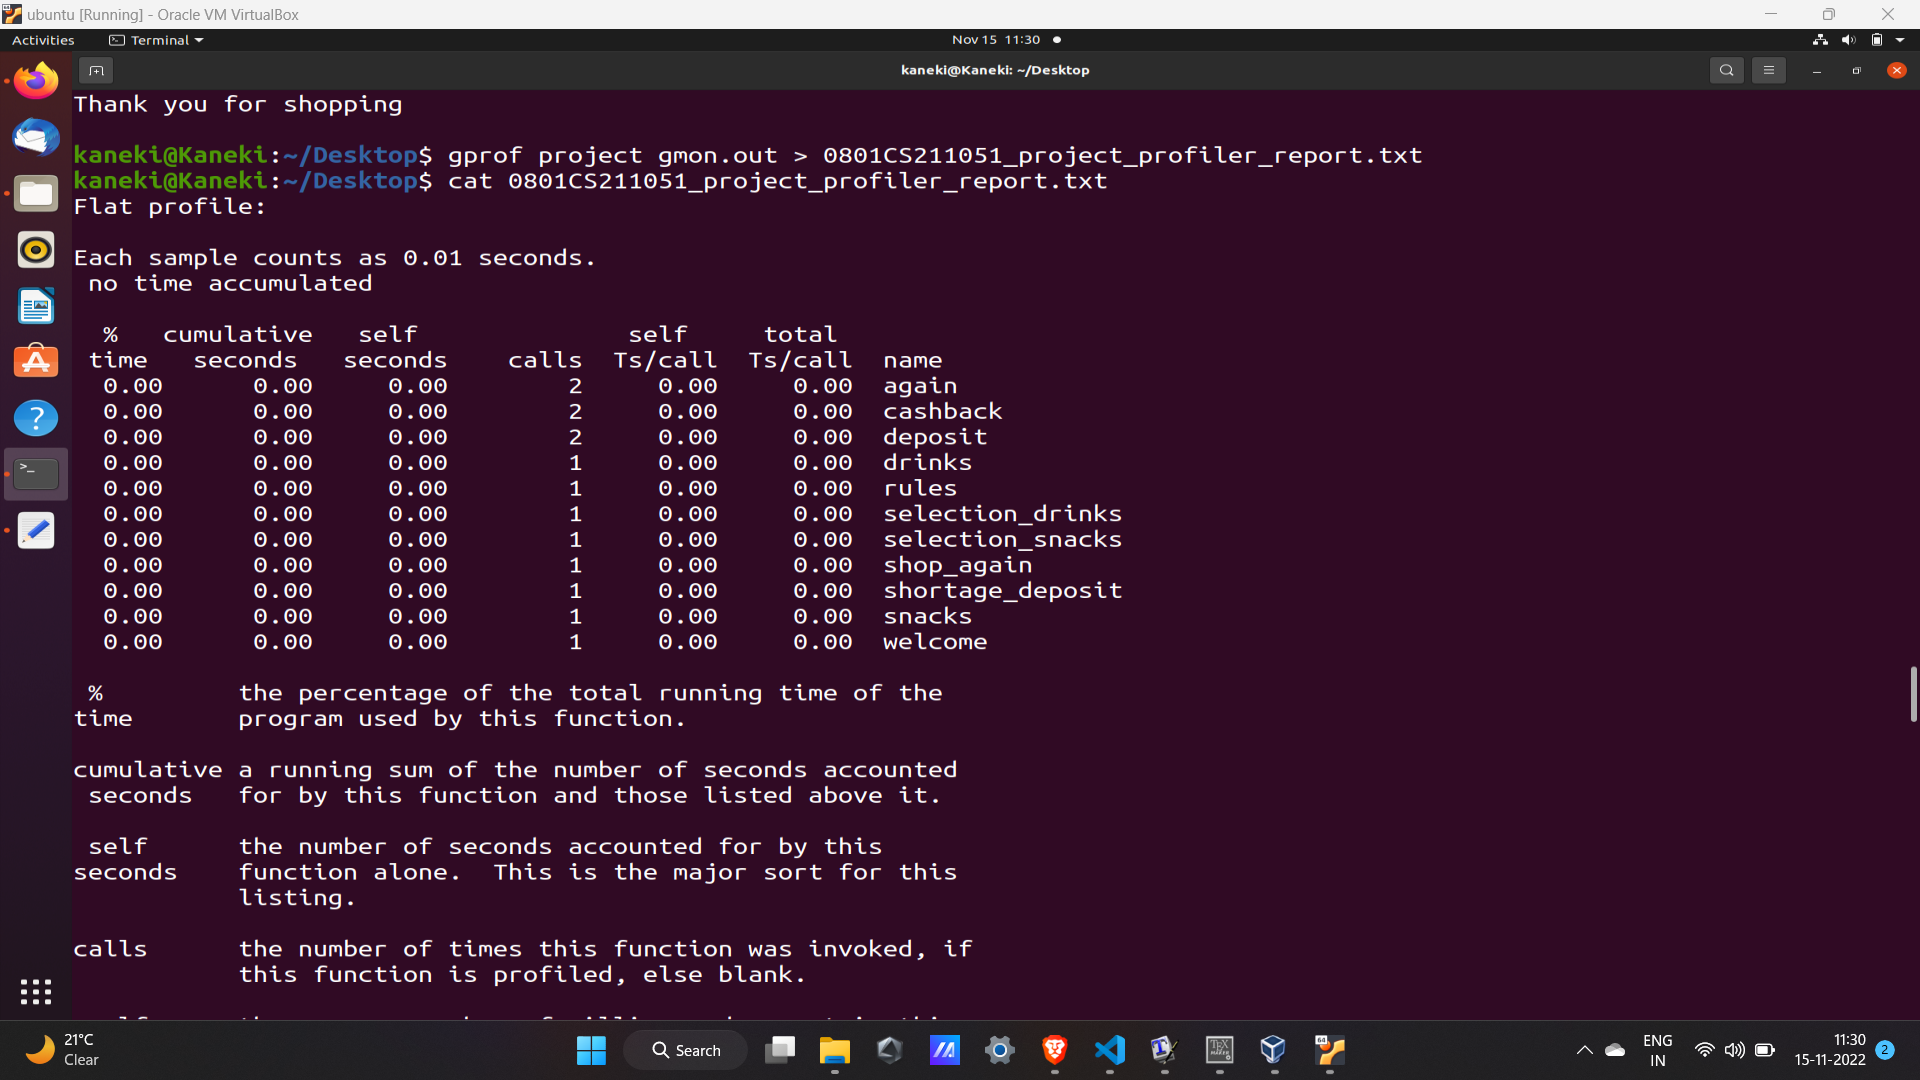
\includegraphics[scale=0.3]{report1}\\
\bigskip
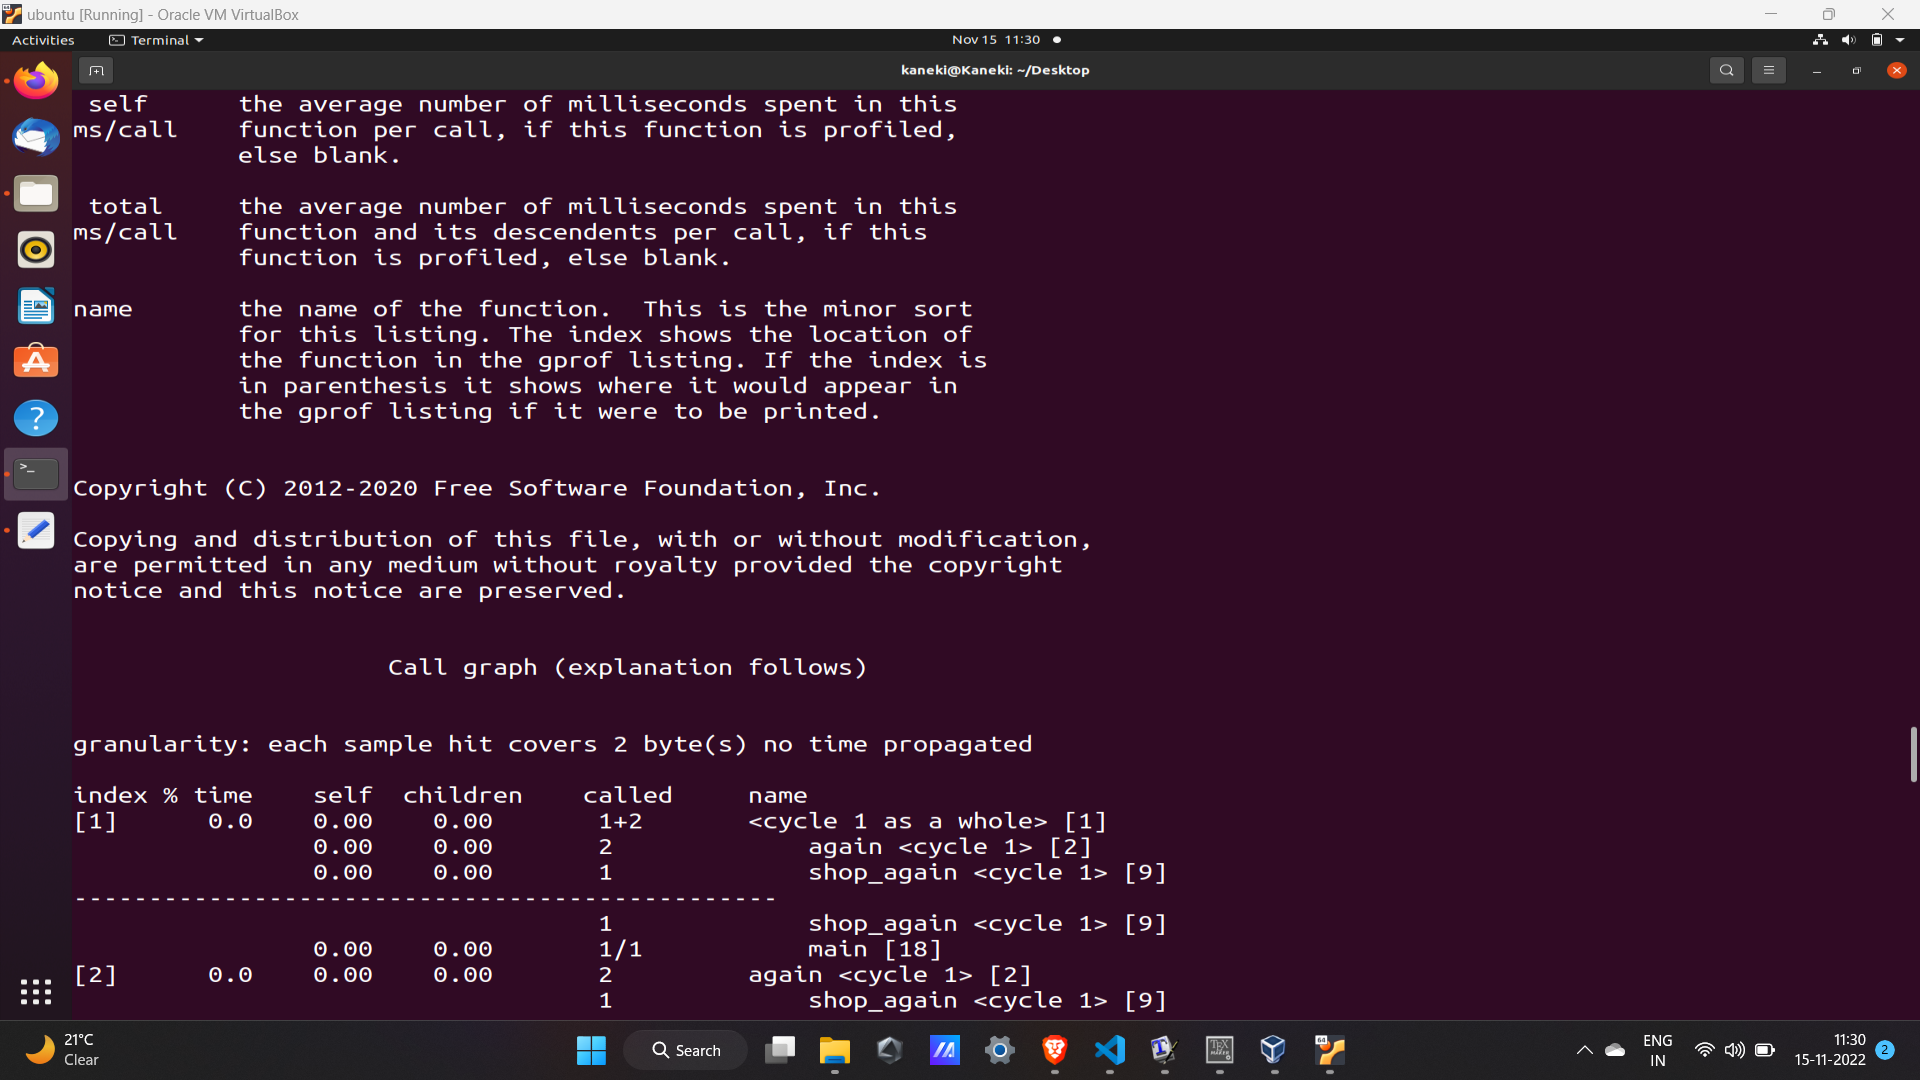
\includegraphics[scale=0.3]{report2}\\
\bigskip
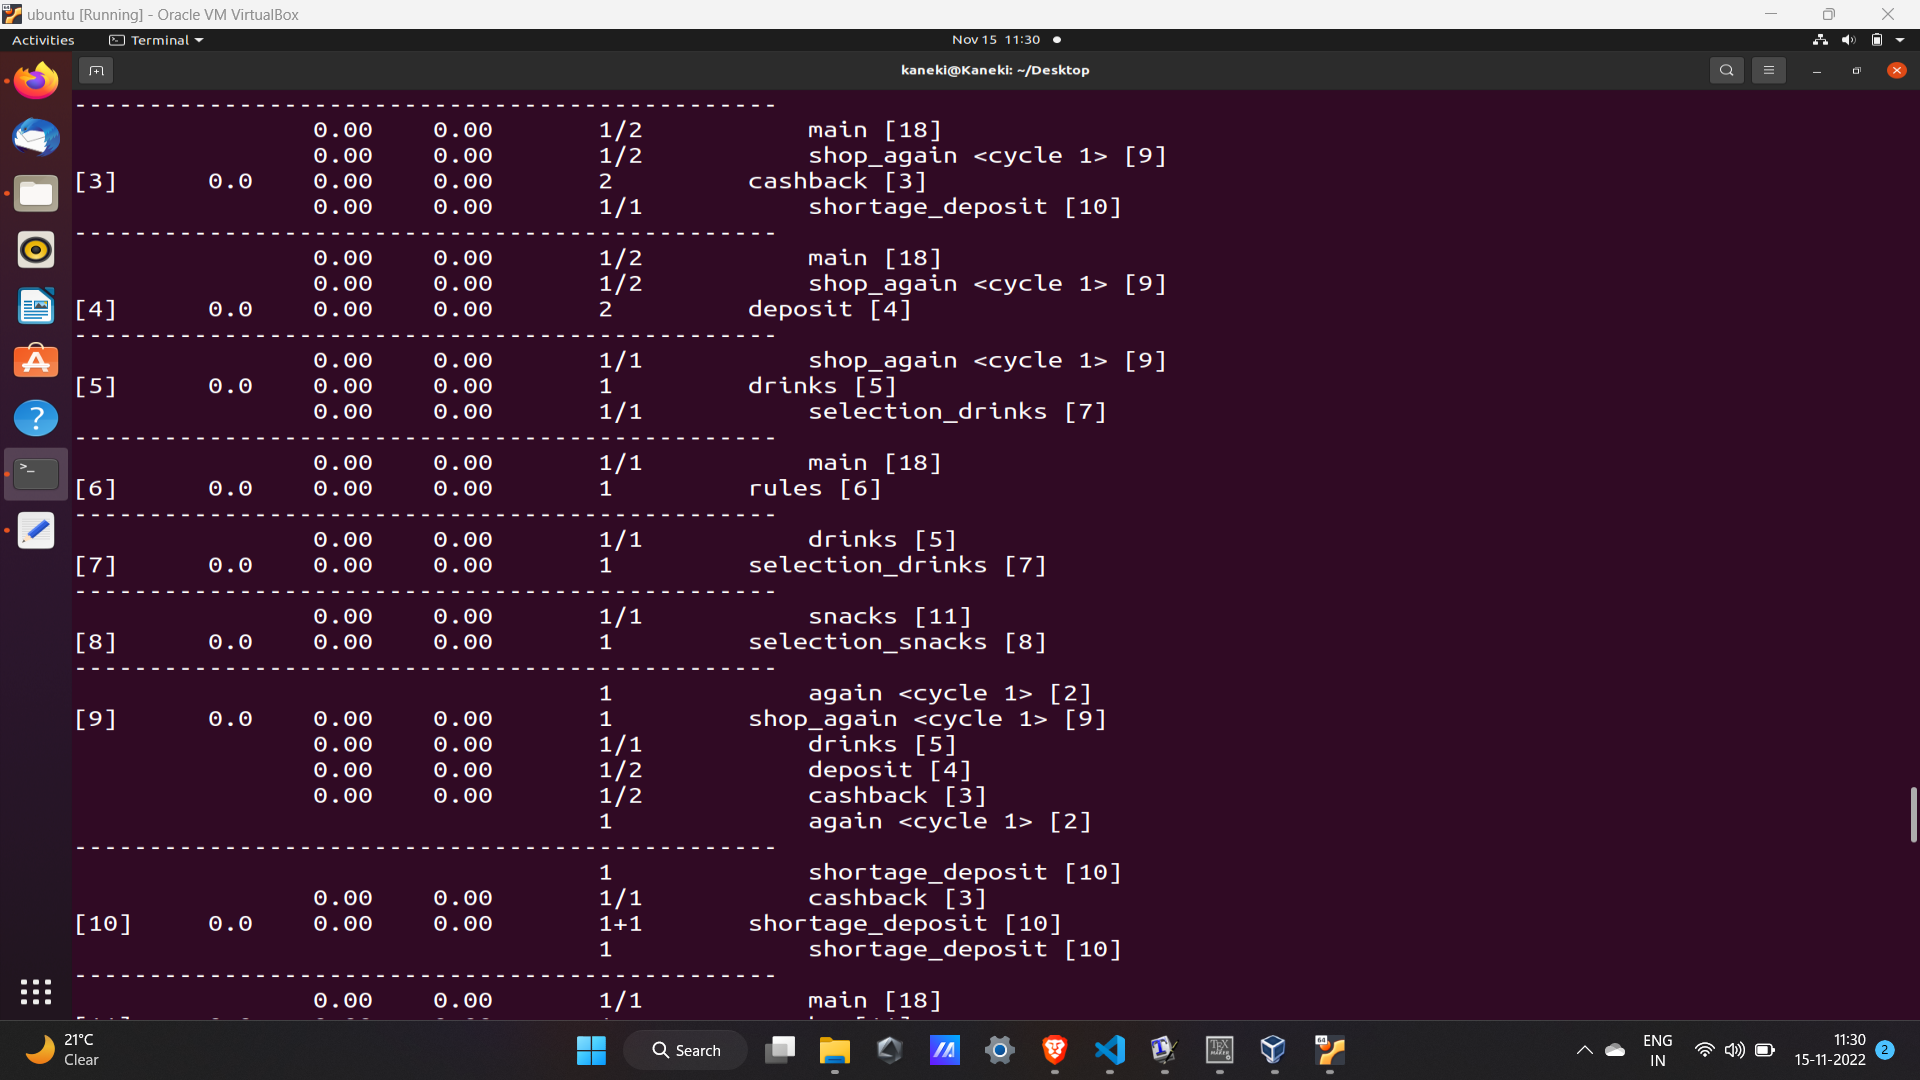
\includegraphics[scale=0.3]{report3}\\
\bigskip
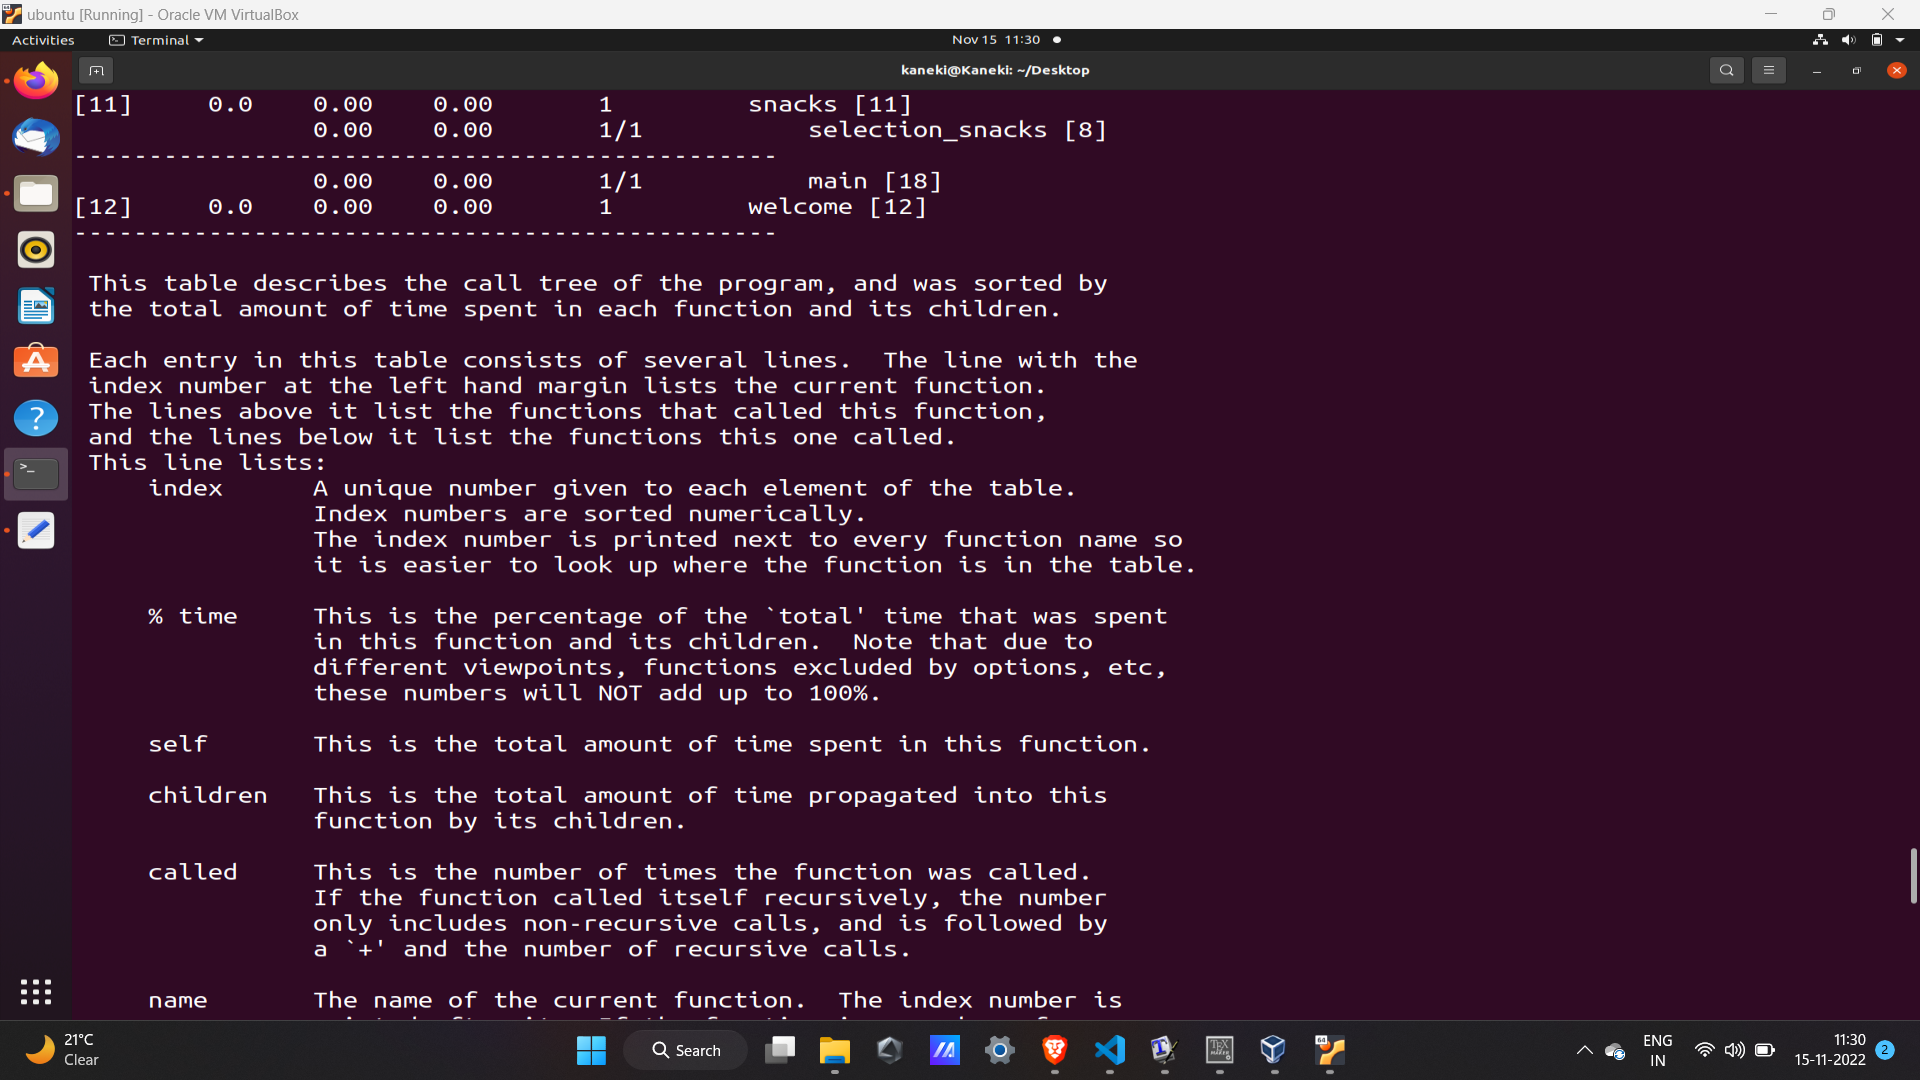
\includegraphics[scale=0.3]{report4}\\
\bigskip
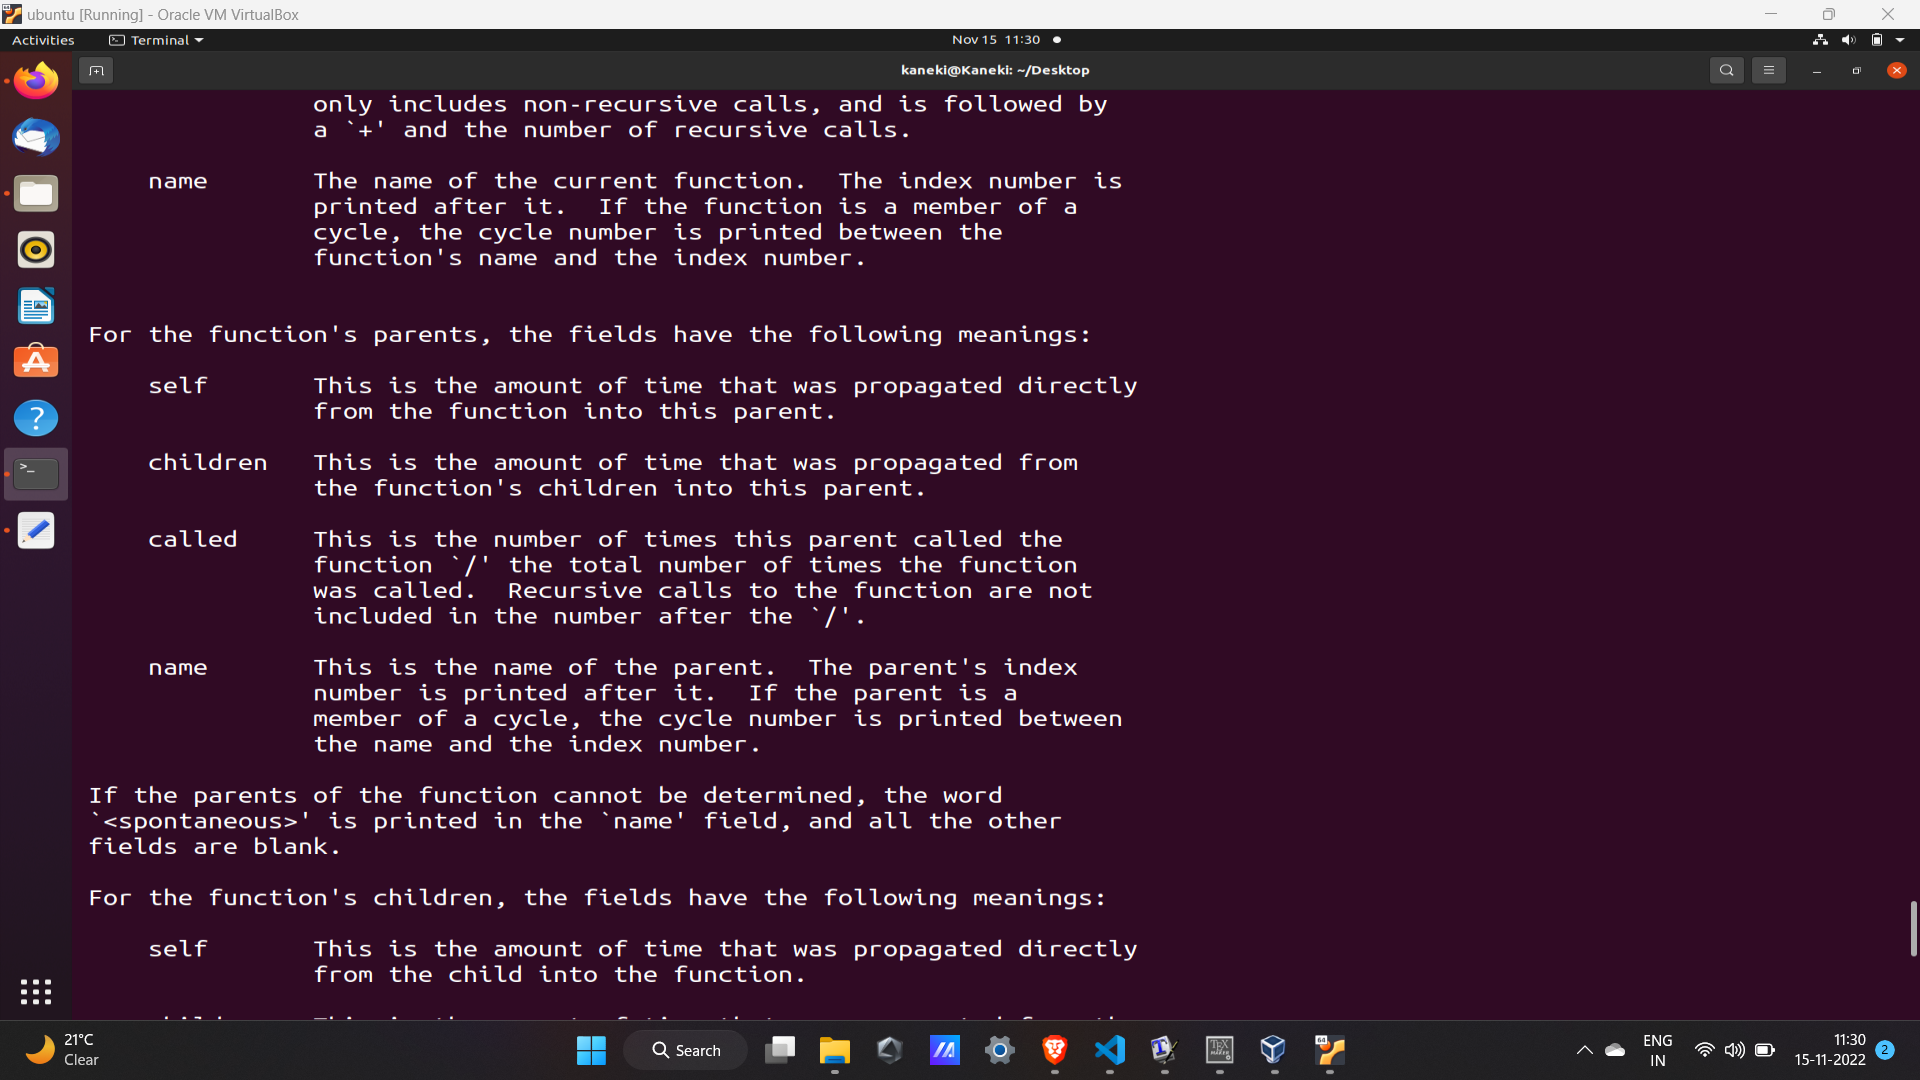
\includegraphics[scale=0.3]{report5}\\
\bigskip
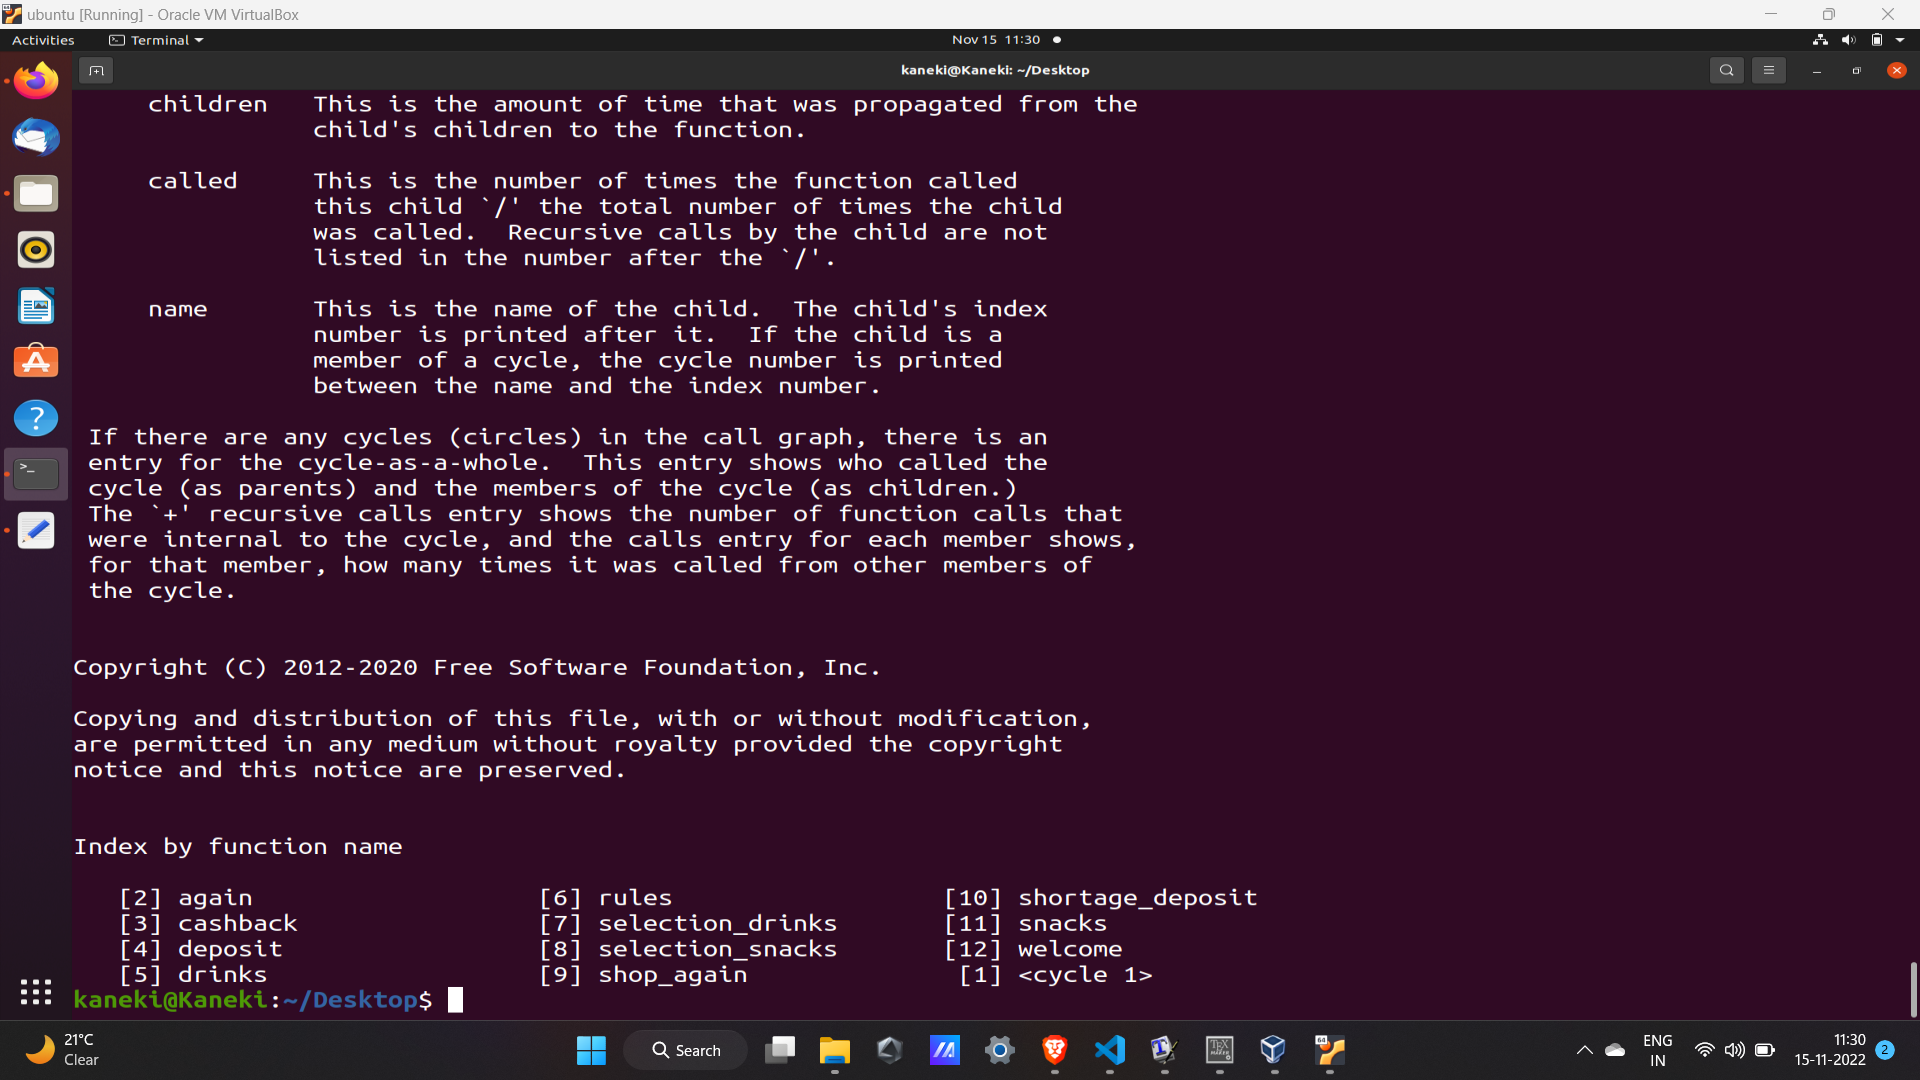
\includegraphics[scale=0.3]{report6}
\end{center}
\newpage
\begin{center}
Debugging\\
\bigskip
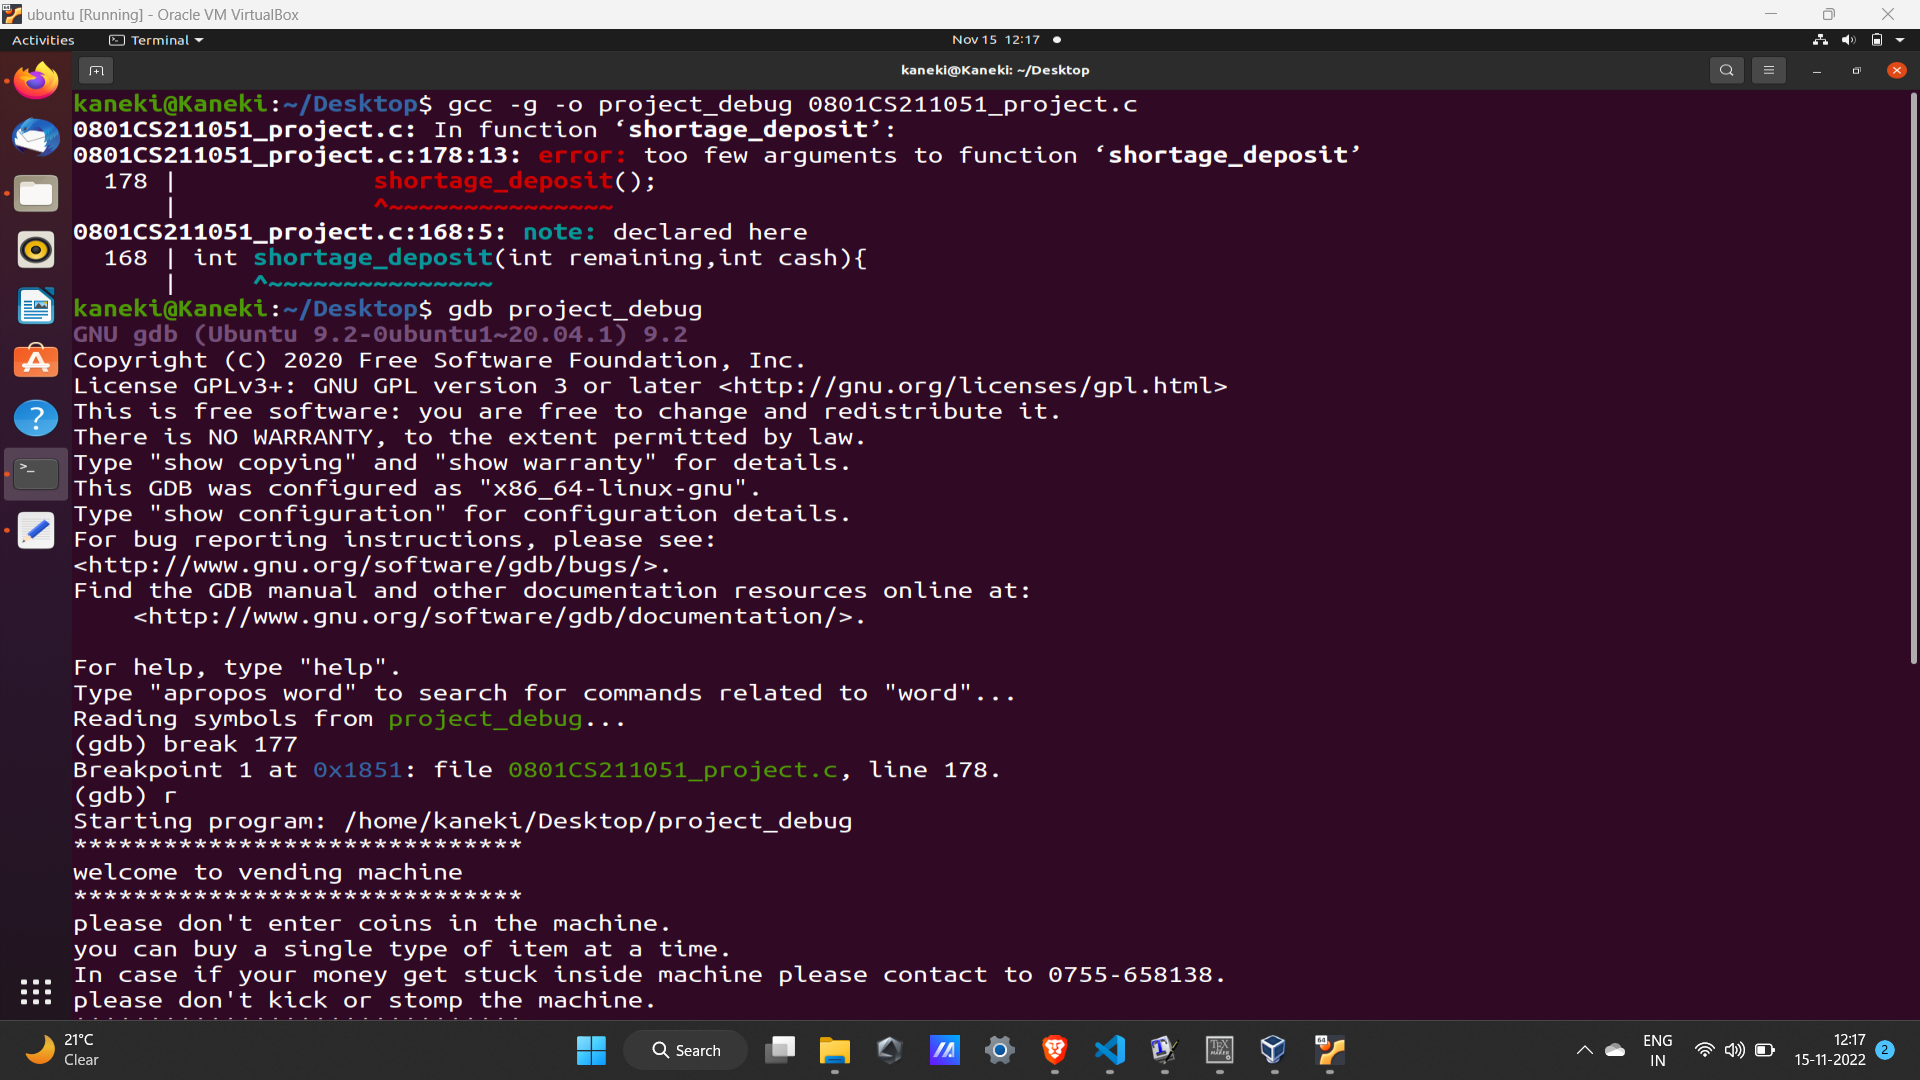
\includegraphics[scale=0.3]{debugging1}\\
\bigskip
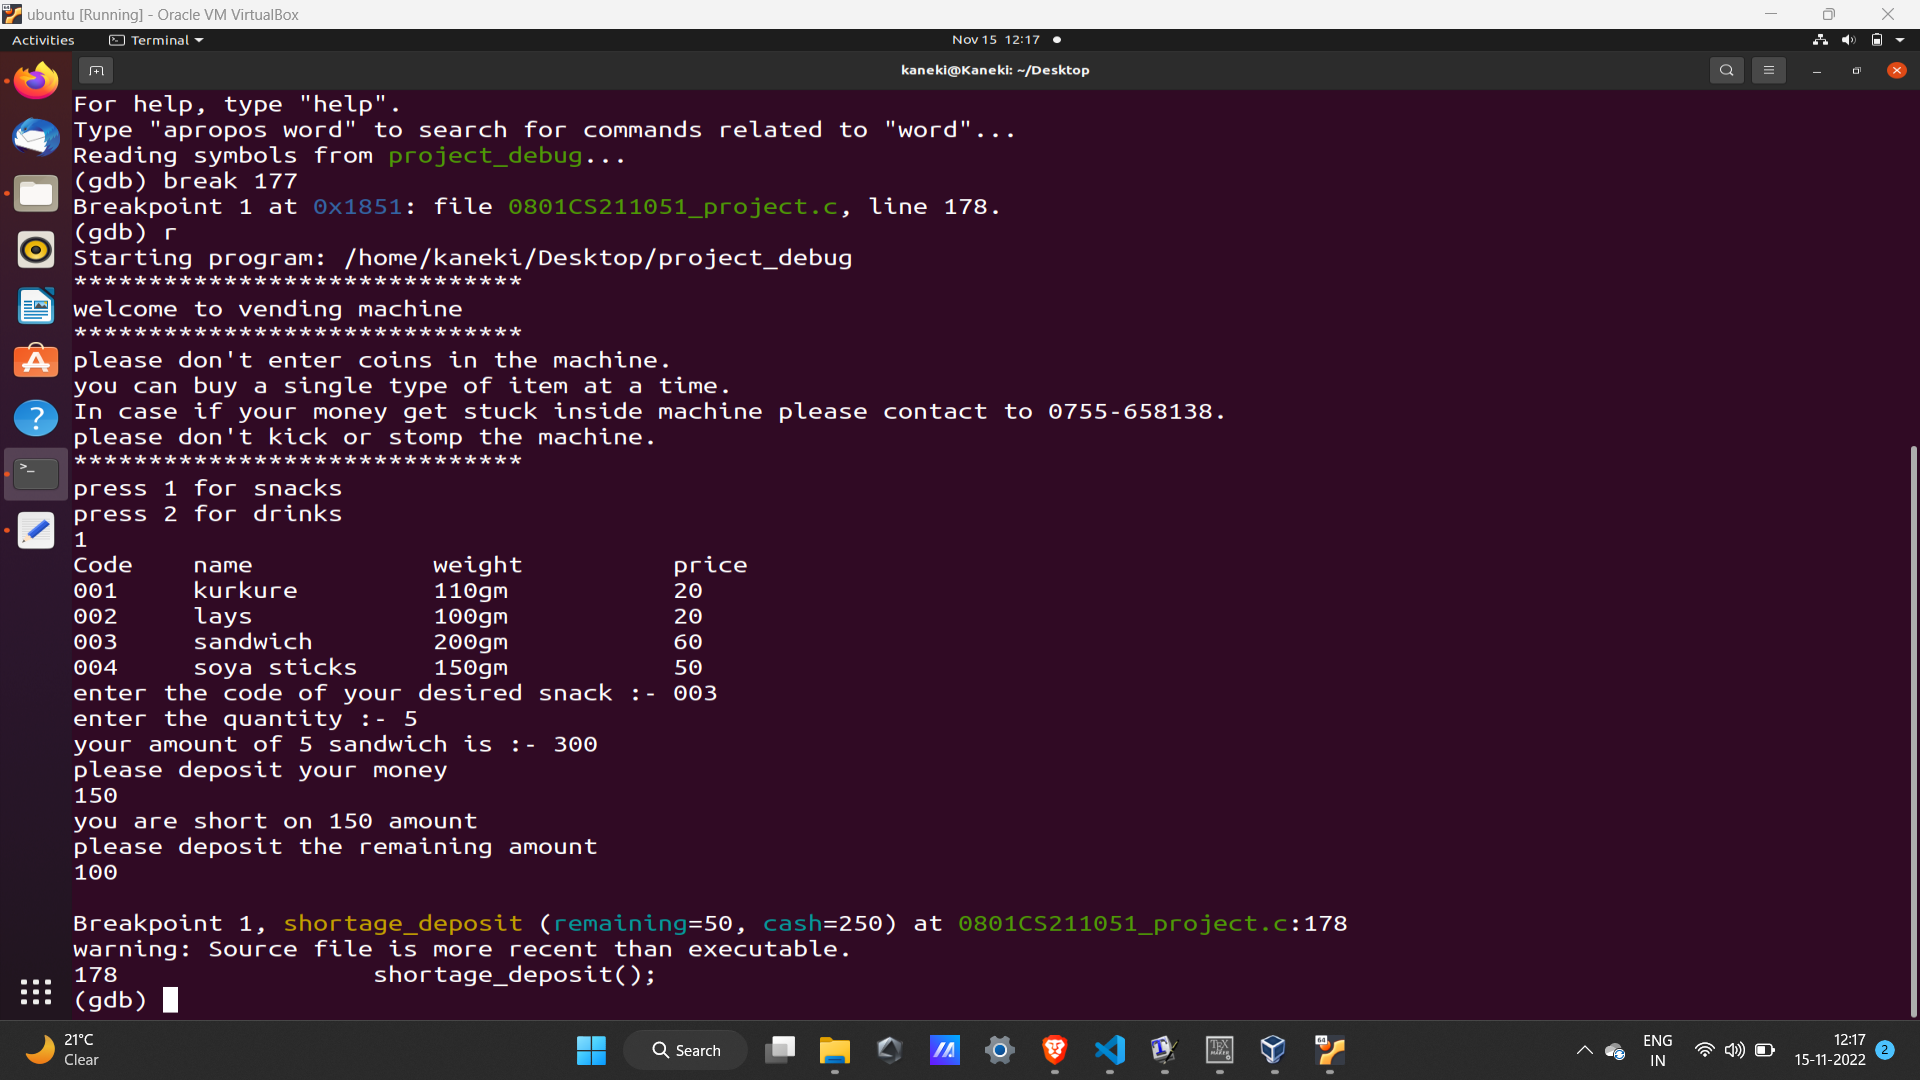
\includegraphics[scale=0.3]{debugging2}
\end{center}
\newpage
\begin{center}
Code in C Language
\end{center}
\#include$\langle stdio.h \rangle$
int amount,purse; //declared global variables \\
void welcome(); //declaring welcome function\\
void rules(); //declaring rules function \\
void snacks(); //declaring snacks function\\
void drinks(); //declaring drinks function\\
int selection\_snacks(); //declaring selection\_snacks function\\
int selection\_drinks(); //declaring selection\_drinks function\\
int deposit(); //declaring deposit function\\
int cashback(int); //declaring cashback function\\
int shortage\_deposit(int,int); //declaring shortage\_deposit function\\
void again(); //declaring again function\\
void shop\_again(); //declaring shop\_again function\\
\bigskip
int main()\{\\
    \hspace*{0.5cm}  int selection,cash;\\
    \hspace*{0.5cm}  welcome();\\
    \hspace*{0.5cm}  rules();\\
    \hspace*{0.5cm}  again:\\
    \hspace*{0.5cm}  printf("\textbackslash n press 1 for snacks \textbackslash n press 2 for drinks \textbackslash n");\\
    \hspace*{0.5cm}  scanf("\%d",\&selection);\\
    \hspace*{0.5cm}  switch (selection)\\   //selection for whether user want snacks or drinks\\
    \hspace*{0.5cm}  \{\\
    \hspace*{0.5cm}  case 1:\\
    \hspace*{0.5cm}  \hspace*{0.5cm}   snacks();  \\//snacks function is called\\
    \hspace*{0.5cm}  \hspace*{0.5cm}  break;\\
    \hspace*{0.5cm}  case 2:\\
    \hspace*{0.5cm}  \hspace*{0.5cm}  drinks();\\   //drinks function is called\\
    \hspace*{0.5cm}  \hspace*{0.5cm} break;\\
    \hspace*{0.5cm}  default:\\
    \hspace*{0.5cm}  \hspace*{0.5cm}   printf("\textbackslash n you pressed wrong number \textbackslash n");\\
    \hspace*{0.5cm}  \hspace*{0.5cm}  goto again;\\   //if user gives wrong input\\
    \hspace*{0.5cm} \}\\
    \hspace*{0.5cm} cash=deposit();\\
    \hspace*{0.5cm}  purse=cashback(cash);\\
    \hspace*{0.5cm}  again();\\
    \hspace*{0.5cm}  return 0;\\ 
\}\\
void welcome()\{\\    //prints welcome message to the user\\
    \hspace*{0.5cm}  for(int i=0;i $\langle$30;i++)\{\\
    \hspace*{0.5cm}  \hspace*{0.5cm}printf("$\ast$");\\
    \hspace*{0.5cm}  \}\\
    \hspace*{0.5cm}  printf("\textbackslash t \textbackslash t \textbackslash n welcome to vending machine \textbackslash n");\\
    \hspace*{0.5cm}  for (int i = 0; i $\langle$ 30; i++)\\
    \hspace*{0.5cm}  \{\\
    \hspace*{0.5cm}  \hspace*{0.5cm}    printf("$\ast$");\\
    \hspace*{0.5cm}  \}\\
\}\\
void rules()\{    //prints rules \\
    \hspace*{0.5cm}  printf("\textbackslash n please don't enter coins in the machine.\textbackslash n");\\
    \hspace*{0.5cm} printf("you can buy a single type of item at a time.\textbackslash n");\\
    \hspace*{0.5cm}  printf("In case if your money get stuck inside machine please contact to 0755-658138.\textbackslash n");\\
    \hspace*{0.5cm}  printf("please don't kick or stomp the machine.\textbackslash n");\\
    \hspace*{0.5cm}  for(int i = 0 ;i$\langle$30;i++)\{\\
    \hspace*{0.5cm}  \hspace*{0.5cm}   printf("$\ast$");\\
    \hspace*{0.5cm}  \}\\
\}\\
void snacks()\{\\    //tells what all snacks are available in vending machine\\
    \hspace*{0.5cm}  printf("Code \textbackslash t name \textbackslash t \textbackslash t weight \textbackslash t \textbackslash t price\textbackslash n");\\
    \hspace*{0.5cm}  printf("001\textbackslash t kurkure \textbackslash t \textbackslash t 110gm \textbackslash t \textbackslash t 20\textbackslash n");\\
    \hspace*{0.5cm}  printf("002 \textbackslash t lays \textbackslash t \textbackslash t 100gm \textbackslash t \textbackslash t 20\textbackslash n");\\
    \hspace*{0.5cm}  printf("003 \textbackslash t sandwich \textbackslash t 200gm \textbackslash t \textbackslash t 60 \textbackslash n");\\
    \hspace*{0.5cm}  printf("004\textbackslash t soya sticks \textbackslash t 150gm \textbackslash t \textbackslash t 50 \textbackslash n");\\
    \hspace*{0.5cm}  amount =selection\_snacks();\\   //selection\_snacks function is called and its returned value is stored in amount\\
\}\\
void drinks()\{\\   //tells what all drinks are available in vending machine\\
    \hspace*{0.5cm}  printf("Code \textbackslash t name \textbackslash t  \textbackslash t weight \textbackslash t  \textbackslash t price \textbackslash n");\\
    \hspace*{0.5cm}  printf("001 \textbackslash t sting \textbackslash t \textbackslash t 200ml \textbackslash t \textbackslash t 20 \textbackslash n");\\
    \hspace*{0.5cm}  printf("002 \textbackslash t amul kool \textbackslash t 150ml \textbackslash t \textbackslash t 20 \textbackslash n");\\
    \hspace*{0.5cm}  printf("003 \textbackslash t coolberg \textbackslash t 500ml \textbackslash t \textbackslash t 60 \textbackslash n");\\
    \hspace*{0.5cm}  printf("004 \textbackslash t pepsi \textbackslash t \textbackslash t 750ml \textbackslash t \textbackslash t 50 \textbackslash n");\\
    \hspace*{0.5cm}  printf("005 \textbackslash t nescafe latte \textbackslash t 300ml \textbackslash t \textbackslash t 45 \textbackslash n");\\
    \hspace*{0.5cm}  printf("006 \textbackslash t red bull \textbackslash t 750ml \textbackslash t \textbackslash t 150 \textbackslash n");\\
    \hspace*{0.5cm}  amount=selection\_drinks();\\    //selection\_drinks function is called and its returned value is stored in amount\\
\}\\
int selection\_snacks()\{\\  //It ask for the code and quantity of the product and calculates total amount of the product \\
    \hspace*{0.5cm}  int code,quantity,total\_amount;\\
    \hspace*{0.5cm}  again\_selection:\\
    \hspace*{0.5cm}  printf("enter the code of your desired snack :- ");\\
    \hspace*{0.5cm}  scanf("\%d",\&code);\\
    \hspace*{0.5cm}  printf("enter the quantity :- ");\\
    \hspace*{0.5cm}  scanf("\%d",\&quantity);\\
    \hspace*{0.5cm}  if (code == 001)\\
    \hspace*{0.5cm}  \{\\
    \hspace*{0.5cm}  \hspace*{0.5cm}total\_amount=20$\ast$quantity;\\
    \hspace*{0.5cm}  \hspace*{0.5cm}printf("your amount of \%d kurkure is :- \%d",quantity,total\_amount);\\
    \hspace*{0.5cm}  \}\\
    \hspace*{0.5cm}  else if (code == 002)\\
    \hspace*{0.5cm}  \{\\
    \hspace*{0.5cm}  \hspace*{0.5cm}total\_amount=20$\ast$quantity;\\
    \hspace*{0.5cm}  \hspace*{0.5cm}printf("your amount of \%d lays is :- \%d",quantity,total\_amount);\\
    \hspace*{0.5cm}  \}\\
    \hspace*{0.5cm}  else if (code == 003)\\
    \hspace*{0.5cm}  \{\\
    \hspace*{0.5cm}  \hspace*{0.5cm}total\_amount=45$\ast$quantity;\\
    \hspace*{0.5cm}  \hspace*{0.5cm}printf("your amount of \%d sandwich is :- \%d",quantity,total\_amount);\\
    \hspace*{0.5cm}  \}\\
    \hspace*{0.5cm}  else if (code == 004)\\
    \hspace*{0.5cm}  \{\\
    \hspace*{0.5cm}  \hspace*{0.5cm}total\_amount=50$\ast$quantity;\\
    \hspace*{0.5cm}  \hspace*{0.5cm}printf("your amount of \%d soya sticks is :- \%d",quantity,total\_amount);\\
    \hspace*{0.5cm}  \}\\
    \hspace*{0.5cm}  else\{\\
    \hspace*{0.5cm}  \hspace*{0.5cm}printf("\textbackslash n you enter wrong code \textbackslash n");\\
    \hspace*{0.5cm}  \hspace*{0.5cm}goto again\_selection;\\ //It ask for the code and quantity of the product and calculates total amount of the product\\
    \hspace*{0.5cm}  \}
    \hspace*{0.5cm}  return total\_amount;\\
\}\\
int selection\_drinks()\{\\   //It ask for the code and quantity of the product and calculates total amount of the product \\
    \hspace*{0.5cm} int code,quantity,total\_amount;\\
    \hspace*{0.5cm}  again\_selection:\\
    \hspace*{0.5cm}  printf("enter the code of your desired drink :- ");\\
    \hspace*{0.5cm}  scanf("\%d",\&code);\\
    \hspace*{0.5cm}  printf("enter the quantity :- ");\\
    \hspace*{0.5cm}  scanf("\%d",\&quantity);
    \hspace*{0.5cm}  if (code == 001)\\
    \hspace*{0.5cm}  \{\\
    \hspace*{0.5cm}  \hspace*{0.5cm}    total\_amount=20$\ast$quantity;\\
    \hspace*{0.5cm}  \hspace*{0.5cm}   printf("your amount of \%d sting is :- \%d",quantity,total\_amount);\\
    \hspace*{0.5cm}  \}\\
    \hspace*{0.5cm}  else if (code == 002)\\
    \hspace*{0.5cm}  \{\\
    \hspace*{0.5cm}  \hspace*{0.5cm}   total\_amount=20$\ast$quantity;\\
    \hspace*{0.5cm}  \hspace*{0.5cm}    printf("your amount of \%d amul kool is :- \%d",quantity,total\_amount);\\
    \hspace*{0.5cm}  \}\\
    \hspace*{0.5cm}  else if (code == 003)\\
    \hspace*{0.5cm}  \{\\
    \hspace*{0.5cm}  \hspace*{0.5cm}   total\_amount=60$\ast$quantity;\\
    \hspace*{0.5cm}  \hspace*{0.5cm}    printf("your amount of \%d coolberg is :- \%d",quantity,total\_amount);\\
    \hspace*{0.5cm}  \}\\
    \hspace*{0.5cm}  else if (code == 004)\\
    \hspace*{0.5cm}  \{\\
    \hspace*{0.5cm}  \hspace*{0.5cm}    total\_amount=50$\ast$quantity;\\
    \hspace*{0.5cm}  \hspace*{0.5cm}    printf("your amount of \%d pepsi is :- %\d",quantity,total\_amount);\\
    \hspace*{0.5cm}  \}\\
    \hspace*{0.5cm}  else if (code == 005)\\
    \hspace*{0.5cm}  \{\\
    \hspace*{0.5cm}  \hspace*{0.5cm}    total\_amount=45$\ast$quantity;\\
    \hspace*{0.5cm}  \hspace*{0.5cm}    printf("your amount of \%d nescafe latte is :- \%d",quantity,total\_amount);\\
    \hspace*{0.5cm}  \}\\
    \hspace*{0.5cm}  else if (code == 006)\\
    \hspace*{0.5cm}  \{\\
    \hspace*{0.5cm}  \hspace*{0.5cm}    total\_amount=150$\ast$quantity;\\
    \hspace*{0.5cm}  \hspace*{0.5cm}   printf("your amount of \%d red bull is :- \%d",quantity,total\_amount);\\
    \hspace*{0.5cm}  \}\\
    \hspace*{0.5cm}  else\{\\
    \hspace*{0.5cm}  \hspace*{0.5cm}    printf("\textbackslash n you enter wrong code \textbackslash n");\\
    \hspace*{0.5cm}  \hspace*{0.5cm}    goto again\_selection;\\  //It ask for the code and quantity of the product and calculates total amount of the product \\
    \hspace*{0.5cm}  \}\\
    \hspace*{0.5cm}  return total\_amount;\\
\}\\
int deposit()\{\\  //it takes deposit from the user and store it in cash variable\\
    \hspace*{0.5cm}  int deposit;\\
    \hspace*{0.5cm}  printf("\textbackslash n please deposit your money \textbackslash n");\\
    \hspace*{0.5cm}  scanf("\%d",\&deposit);\\
    \hspace*{0.5cm}  return deposit;\\
\}\\
/$\ast$it calculates that is there any shortage of money in the deposited amount and tells the left amount in the purse. It returns
remaining$\ast$-1 to purse variable in the main function. $\ast$/\\
int cashback(int cash)\{\\
    \hspace*{0.5cm}  int remaining;\\
    \hspace*{0.5cm}  remaining = amount - cash;\\
    \hspace*{0.5cm}  if(remaining$\rangle$0)\{\\
    \hspace*{0.5cm}  \hspace*{0.5cm}   remaining=shortage\_deposit(remaining,cash);\\
    \hspace*{0.5cm}  \hspace*{0.5cm}\}\\
    \hspace*{0.5cm}  printf("\textbackslash n you got \%d amount left \textbackslash n",remaining$\ast$-1);\\
    \hspace*{0.5cm}  return remaining$\ast$-1;\\
\}\\
/$\ast$it tells the user on how much money he is short on and takes the remaining amount and then also if the user is in shortage 
it will go in recursion until the amount = deposit.it returns the remaining to function cashback.$\ast$/\\
int shortage\_deposit(int remaining,int cash)\{\\
    \hspace*{0.5cm}  int shortage,left;\\
    \hspace*{0.5cm}  remaining=cash - amount;\\
    \hspace*{0.5cm}  printf("you are short on \%d amount \textbackslash n",remaining$\ast$-1);\\
    \hspace*{0.5cm}  printf("please deposit the remaining amount \textbackslash n");\\
    \hspace*{0.5cm}  scanf("\%d",\&shortage);\\
    \hspace*{0.5cm}  remaining = (remaining$\ast$-1)-shortage;\\
    \hspace*{0.5cm}  cash = cash+shortage;\\
    \hspace*{0.5cm}  if (remaining$\rangle$0)\\
    \hspace*{0.5cm}  \{\\
    \hspace*{0.5cm}  \hspace*{0.5cm}shortage\_deposit(remaining,cash);\\
    \hspace*{0.5cm}  \}\\
    \hspace*{0.5cm}  else\{\\
    \hspace*{0.5cm}  \hspace*{0.5cm}return remaining;\\
    \hspace*{0.5cm}  \}\\
\}\\
/$\ast$it asks the that does he want to buy again anything and if the user wants to buy something then shop\_again 
function will be called else thank you message will be printed.$\ast$/\\
void again()\{\\
    \hspace*{0.5cm}  int response;\\
    \hspace*{0.5cm}  try\_again:\\
    \hspace*{0.5cm}  printf("press 1 if you want to buy something else \textbackslash n ");\\
    \hspace*{0.5cm}  printf("\textbackslash n pres 2 if you want to quit ");\\
    \hspace*{0.5cm}  scanf("\%d",\&response);\\
    \hspace*{0.5cm}  switch (response)\\
    \hspace*{0.5cm}  \{\\
    \hspace*{0.5cm}  case 1:\\
    \hspace*{0.5cm}  \hspace*{0.5cm}   shop\_again();\\
    \hspace*{0.5cm}  \hspace*{0.5cm}   break;\\
    \hspace*{0.5cm}  case 2:\\
    \hspace*{0.5cm}  for (int i = 0; i $\langle$ 30; i++)\\
    \hspace*{0.5cm}  \{\\
    \hspace*{0.5cm}  \hspace*{0.5cm}       printf("$\ast$");\\
    \hspace*{0.5cm}  \}\\
    \hspace*{0.5cm}  printf("\textbackslash n Thank you for shopping \textbackslash n");\\
    \hspace*{0.5cm}  printf("\textbackslash n please visit us again \textbackslash n");\\
    \hspace*{0.5cm}  for (int i = 0; i $\langle$ 30; i++)\\
    \hspace*{0.5cm}  \{\\
    \hspace*{0.5cm}  \hspace*{0.5cm}printf("$\ast$");\\
    \hspace*{0.5cm}  \}\\
    \hspace*{0.5cm}  break;\\
    \hspace*{0.5cm}  default:\\
    \hspace*{0.5cm}  \hspace*{0.5cm}printf("you pressed wrong number");\\
    \hspace*{0.5cm   \hspace*{0.5cm}}goto try\_again;\\
    \hspace*{0.5cm}  \hspace*{0.5cm}break;\\
    \hspace*{0.5cm}  \}\\\
\}\\
/$\ast$ it calls all the function again except welcome and rules function and add the last remaining amount in 
the purse for future purchases $\ast$/\\
void shop\_again()\{\\
    \hspace*{0.5cm}  int selection,cash;\\
    \hspace*{0.5cm}  again:\\
    \hspace*{0.5cm}  printf("\textbackslash n press 1 for snacks \textbackslash n press 2 for drinks \textbackslash n");\\
    \hspace*{0.5cm}  scanf("\%d",\&selection);\\
    \hspace*{0.5cm}  switch (selection)\\
    \hspace*{0.5cm}  \{\\
    \hspace*{0.5cm}  case 1:\\
    \hspace*{0.5cm}  \hspace*{0.5cm}    snacks();\\
    \hspace*{0.5cm}  \hspace*{0.5cm}    break;\\
    \hspace*{0.5cm}  case 2:\\
    \hspace*{0.5cm}  \hspace*{0.5cm}   drinks();\\
    \hspace*{0.5cm}  \hspace*{0.5cm}   break;\\
    \hspace*{0.5cm}  default:\\
    \hspace*{0.5cm}  \hspace*{0.5cm}    printf("\textbackslash n you pressed wrong number \textbackslash n");\\
    \hspace*{0.5cm}  \hspace*{0.5cm}   goto again;\\
    \hspace*{0.5cm}  \}\\
    \hspace*{0.5cm}  cash=deposit()+purse;\\
    \hspace*{0.5cm}  cashback(cash);\\
    \hspace*{0.5cm}  again();\\
\}
\newpage
\begin{center}
Output of the code\\
\bigskip
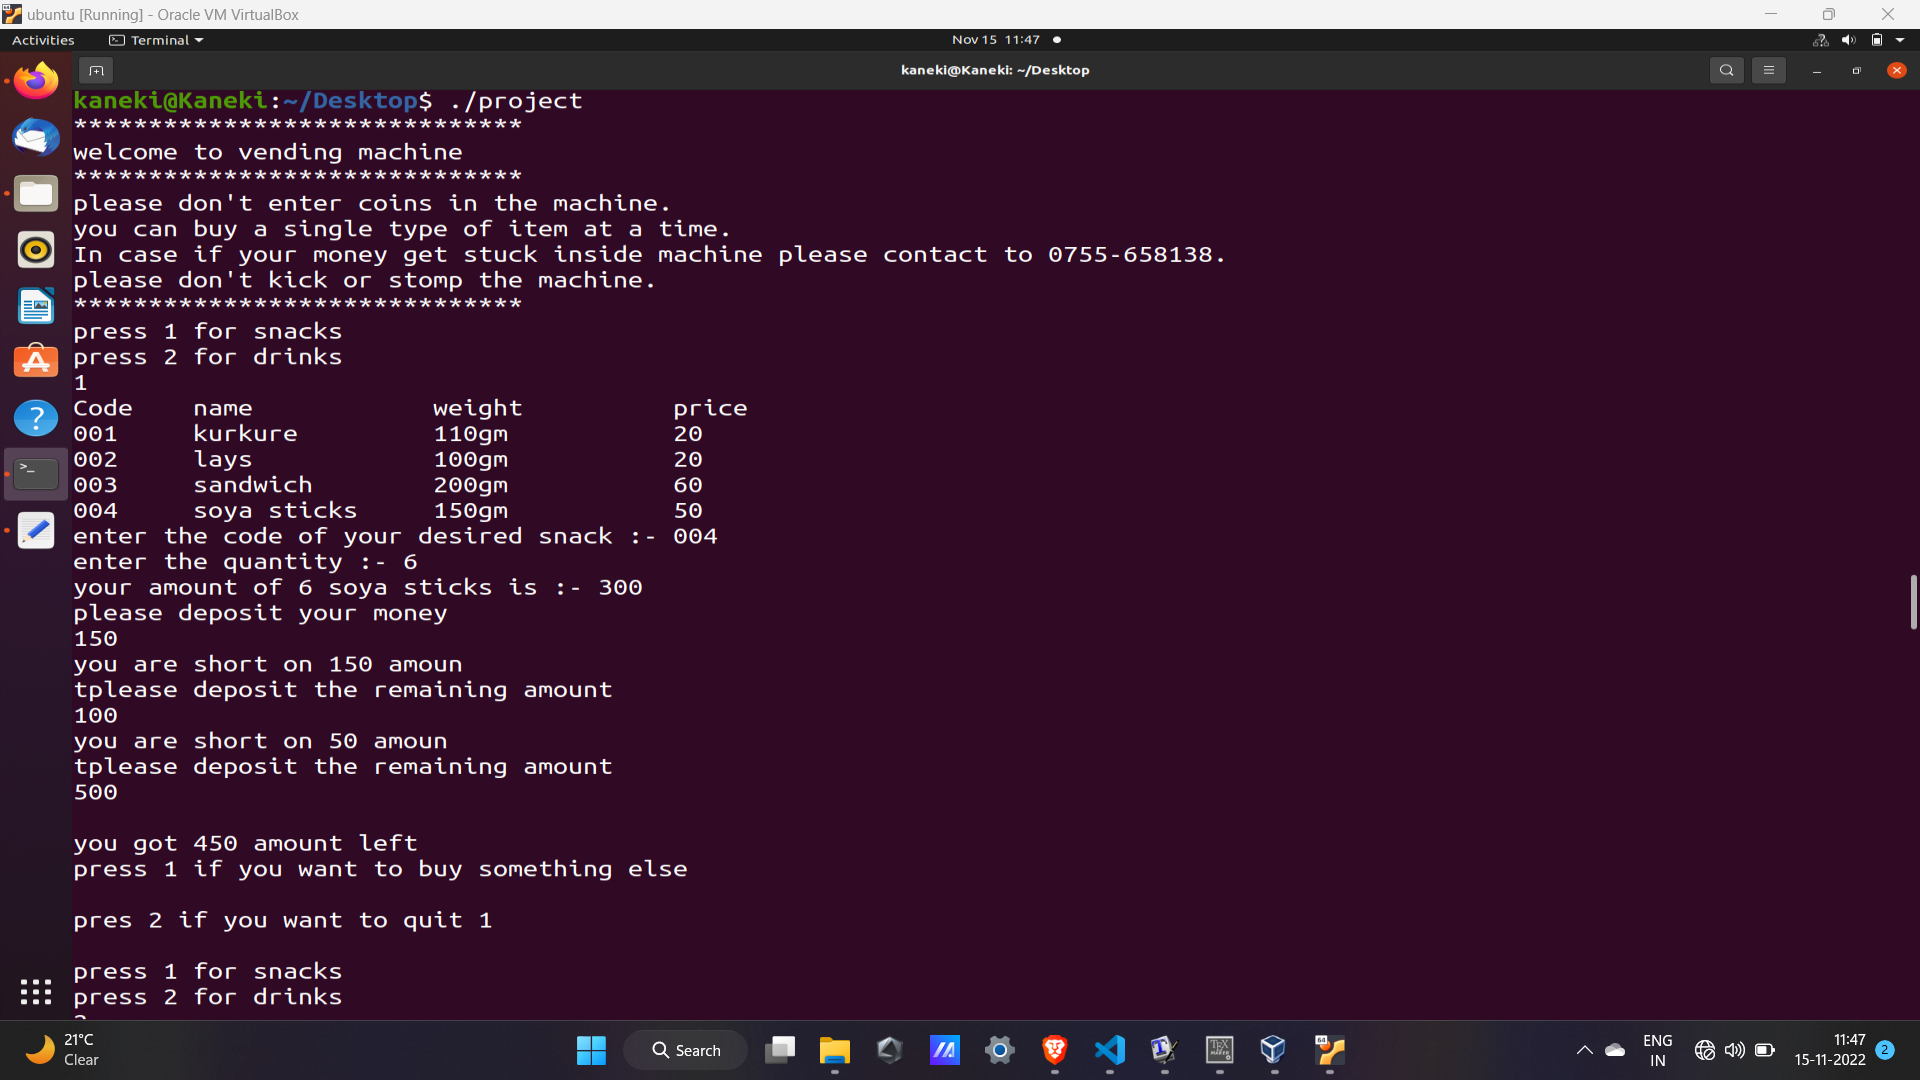
\includegraphics[scale=0.3]{code output1}\\
\bigskip
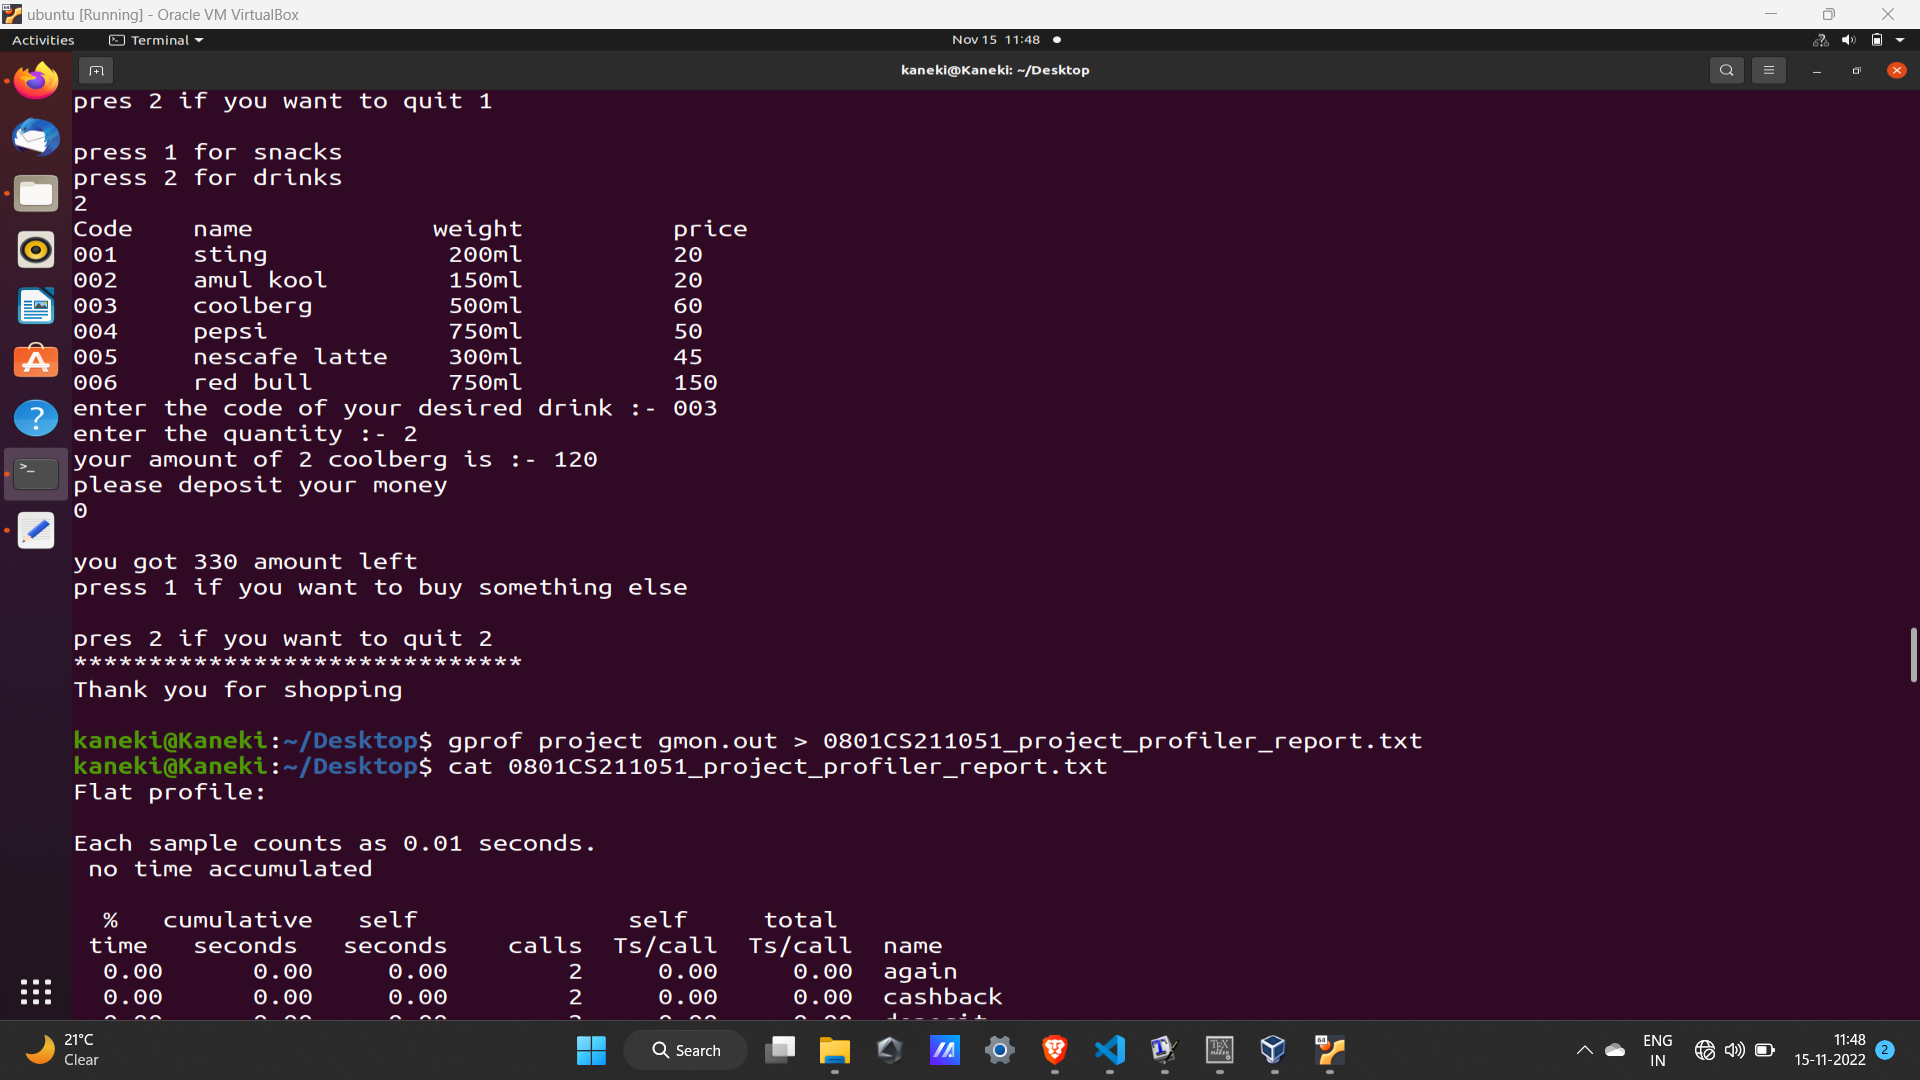
\includegraphics[scale=0.3]{code output2}
\end{center}
\newpage
\begin{center}
Code in Python Language\\
\bigskip
\end{center}
global amount\\
global purse\\
purse = 0\\
def welcome():\\\#prints welcome message to the user\\
\hspace*{0.5cm}    for i in range (0,30):\\
\hspace*{0.5cm}\hspace*{0.5cm}        print("$\ast$",end='')\\
\hspace*{0.5cm}    print(" \textbackslash n welcome to vending machine \textbackslash n")\\
\hspace*{0.5cm}    for i in range (0,30):\\
\hspace*{0.5cm}\hspace*{0.5cm}        print("$\ast$",end='')\\
\bigskip
def rules():\\ \#prints rules \\
\hspace*{0.5cm}    print(" \textbackslash n please don't enter coins in the machine.\textbackslash n ")\\
\hspace*{0.5cm}    print("you can buy a single type of item at a time.\textbackslash n ")\\
\hspace*{0.5cm}    print("In case if your money get stuck inside machine please contact to 0755-658138. \textbackslash n ")\\
\hspace*{0.5cm}    print("please don't kick or stomp the machine. \textbackslash t ")\\
\bigskip
def snack():\\  \#tells what all snacks are available in vending machine\\
\hspace*{0.5cm}    print("Code\textbackslash t name\textbackslash t \textbackslash t weight \textbackslash t \textbackslash t price \textbackslash n ")\\
\hspace*{0.5cm}    print("101 \textbackslash t kurkure \textbackslash t \textbackslash t 110gm \textbackslash t \textbackslash t 20 \textbackslash n")\\
\hspace*{0.5cm}    print("102 \textbackslash t lays \textbackslash t \textbackslash t 100gm \textbackslash t \textbackslash t 20 \textbackslash n")\\
\hspace*{0.5cm}    print("103 \textbackslash t sandwich \textbackslash t 200gm \textbackslash t \textbackslash t 60 \textbackslash n")\\
\hspace*{0.5cm}    print("104 \textbackslash t soya sticks \textbackslash t 150gm \textbackslash t \textbackslash t 50 \textbackslash n")\\
\hspace*{0.5cm}    amount = selection\_snacks()\\  \#selection\_snacks function is called and its returned value is stored in amount\\
\hspace*{0.5cm}    return amount\\
\bigskip
def selection\_snacks():\\  \#It ask for the code and quantity of the product and calculates total amount of the product \\
\hspace*{0.5cm}    total\_amount=0\\
\hspace*{0.5cm}    code = int(input("enter the code of your desired snack \textbackslash n "))\\
\hspace*{0.5cm}    quantity=int(input("enter the quantity \textbackslash n"))\\
\hspace*{0.5cm}    if code == 101:\\
\hspace*{0.5cm}\hspace*{0.5cm}        total\_amount = 20$\ast$quantity\\
\hspace*{0.5cm}\hspace*{0.5cm}        print("your amount for ",quantity,"kurkure is ",total\_amount)\\
\hspace*{0.5cm}    elif code == 102:\\
\hspace*{0.5cm}\hspace*{0.5cm}        total\_amount=20$\ast$quantity\\
\hspace*{0.5cm}\hspace*{0.5cm}        print("your amount for ",quantity,"lays is ",total\_amount)\\
\hspace*{0.5cm}    elif code == 103:\\
\hspace*{0.5cm}\hspace*{0.5cm}        total\_amount=60$\ast$quantity\\
\hspace*{0.5cm}\hspace*{0.5cm}        print("your amount for ",quantity,"sandwich is ",total\_amount)\\
\hspace*{0.5cm}    elif code == 104:\\
\hspace*{0.5cm}\hspace*{0.5cm}        total\_amount=50$\ast$quantity\\
\hspace*{0.5cm}\hspace*{0.5cm}        print("your amount for ",quantity,"soya sticks is ",total\_amount)\\ 
\hspace*{0.5cm}    return total\_amount\\
\bigskip
def drinks():\\  \#tells what all drinks are available in vending machine\\
\hspace*{0.5cm}    print("Code \textbackslash t name \textbackslash t \textbackslash t weight \textbackslash t \textbackslash t price\textbackslash n")\\
\hspace*{0.5cm}    print("101 \textbackslash t sting \textbackslash t \textbackslash t 200ml \textbackslash t \textbackslash t 20  \textbackslash n")\\
\hspace*{0.5cm}    print("102 \textbackslash t amul kool \textbackslash t 150ml \textbackslash t \textbackslash t 20 \textbackslash n")\\
\hspace*{0.5cm}    print("103 \textbackslash t coolberg \textbackslash t  500ml \textbackslash t \textbackslash t 60 \textbackslash n")\\
\hspace*{0.5cm}    print("104 \textbackslash t pepsi \textbackslash t \textbackslash t 750ml \textbackslash t \textbackslash t 50 \textbackslash n")\\
\hspace*{0.5cm}    print("105 \textbackslash t nescafe latte  \textbackslash t  300ml \textbackslash t \textbackslash t 45 \textbackslash n")\\
\hspace*{0.5cm}    print("106 \textbackslash t red bull \textbackslash t 750ml \textbackslash t \textbackslash t 150 \textbackslash n")\\
\hspace*{0.5cm}    amount=selection\_drinks()\\  \#selection\_drinks function is called and its returned value is stored in amount\\
 \hspace*{0.5cm}   return amount\\
\bigskip
def selection\_drinks():\\  \#It ask for the code and quantity of the product and calculates total amount of the product \\
\hspace*{0.5cm}    total\_amount=0\\
\hspace*{0.5cm}    code = int(input(" \textbackslash n enter the code of your desired drink \textbackslash n"))\\
\hspace*{0.5cm}    quantity=int(input("\textbackslash n enter the quantity \textbackslash n"))\\
\hspace*{0.5cm}    if code == 101:\\
\hspace*{0.5cm}\hspace*{0.5cm}        total\_amount = 20$\ast$quantity\\
\hspace*{0.5cm}\hspace*{0.5cm}        print("your amount for ",quantity,"sting is ",total\_amount)\\
\hspace*{0.5cm}    elif code == 102:\\
\hspace*{0.5cm}\hspace*{0.5cm}        total\_amount=20$\ast$quantity\\
\hspace*{0.5cm}\hspace*{0.5cm}        print("your amount for ",quantity,"amul kool is ",total\_amount)\\
\hspace*{0.5cm}    elif code == 103:\\
\hspace*{0.5cm}\hspace*{0.5cm}        total\_amount=60$\ast$quantity\\
\hspace*{0.5cm}\hspace*{0.5cm}        print("your amount for ",quantity,"coolberg is ",total\_amount)\\
\hspace*{0.5cm}    elif code == 104:\\
\hspace*{0.5cm}\hspace*{0.5cm}        total\_amount=50$\ast$quantity\\ 
\hspace*{0.5cm}\hspace*{0.5cm}        print("your amount for ",quantity,"pepsi is ",total\_amount)\\ 
\hspace*{0.5cm}    elif code == 105:\\
\hspace*{0.5cm}\hspace*{0.5cm}        total\_amount=45$\ast$quantity\\
\hspace*{0.5cm}\hspace*{0.5cm}        print("your amount for ",quantity,"nescafe latte is ",total\_amount)\\
\hspace*{0.5cm}    elif code == 106:\\
\hspace*{0.5cm}\hspace*{0.5cm}        total\_amount=150$\ast$quantity\\
\hspace*{0.5cm}\hspace*{0.5cm}        print("your amount for ",quantity,"red bull is ",total\_amount)\\
\hspace*{0.5cm}    return total\_amount\\
\bigskip        
def deposit():\\  \#it takes deposit from the user and store it in cash variable\\
\hspace*{0.5cm}    deposit = int(input("please deposit your money " ))\\
\hspace*{0.5cm}    return deposit\\
\bigskip
"""\\
It calculates that is there any shortage of money in the deposited amount and tells the left amount in the purse. It returns
remaining$\ast$-1 to purse variable in the main function.\\
"""\\
def cashback(cash,amount):\\
\hspace*{0.5cm}    remaining:any\\
\hspace*{0.5cm}    left=0\\
\hspace*{0.5cm}    remaining=amount-cash\\
\hspace*{0.5cm}    if remaining$\rangle$0:\\
\hspace*{0.5cm}\hspace*{0.5cm}        remaining=shortage\_deposit(remaining,cash)\\
\hspace*{0.5cm}    left=remaining$\ast$-1\\
\hspace*{0.5cm}    print("\textbackslash n you got ",left,"amount left in your purse")\\
\hspace*{0.5cm}   return left\\
\bigskip
"""\\
It tells the user on how much money he is short on and takes the remaining amount and then also if the user is in shortage 
it will go in recursion until the amount = deposit.it returns the remaining to function cashback.\\
"""\\  
def shortage\_deposit(remaining,cash):\\
\hspace*{0.5cm}    shortage:any\\
\hspace*{0.5cm}    purse\\
\hspace*{0.5cm}    remaining=cash-amount\\
\hspace*{0.5cm}    print("you are short on ",remaining$\ast$-1,"amount \textbackslash n")\\
\hspace*{0.5cm}    shortage = int(input("please deposit the  remaining amount \textbackslash n"))\\
\hspace*{0.5cm}    remaining = (remaining$\ast$-1)-shortage\\
\hspace*{0.5cm}    cash=cash+shortage\\
\hspace*{0.5cm}   if remaining$\rangle$0:\\
\hspace*{0.5cm}\hspace*{0.5cm}        shortage\_deposit(remaining,cash)\\
\hspace*{0.5cm}    else:\\
\hspace*{0.5cm}\hspace*{0.5cm}        return remaining\\
\bigskip        
"""\\
it asks the that does he want to buy again anything and if the user wants to buy something then shop\_again 
function will be called else thank you message will be printed.\\
"""\\ 
def again(purse):\\
\hspace*{0.5cm}    response:any\\
\hspace*{0.5cm}    print("press 1 if you want to buy something else \textbackslash n")\\
\hspace*{0.5cm}    print("press 2 if you want to quit")\\
\hspace*{0.5cm}    response=int(input())\\
\hspace*{0.5cm}    if response == 1:\\
\hspace*{0.5cm}\hspace*{0.5cm}        shop\_again(purse)\\
\hspace*{0.5cm}    else:\\
\hspace*{0.5cm}\hspace*{0.5cm}        for i in range (0,30):\\
\hspace*{0.5cm}\hspace*{0.5cm}\hspace*{0.5cm}            print("$\ast$",end='')\\
\hspace*{0.5cm}\hspace*{0.5cm}        print("\textbackslash n Thank you for shopping \textbackslash n")\\
\hspace*{0.5cm}\hspace*{0.5cm}        print("\textbackslash n Please visit us again \textbackslash n")\\
\hspace*{0.5cm}\hspace*{0.5cm}        for i in range(0,30):\\
\hspace*{0.5cm}\hspace*{0.5cm}\hspace*{0.5cm}            print("$\ast$",end='')\\
\bigskip
"""\\
It calls all the function again except welcome and rules function and add the last remaining amount in 
the purse for future purchases\\
"""\\
def shop\_again(purse):\\
\hspace*{0.5cm}    selection:any\\
\hspace*{0.5cm}    cash:any\\
\hspace*{0.5cm}    print("\textbackslash n press 1 for snacks and press 2 for drinks \textbackslash n")\\
\hspace*{0.5cm}    selection=int(input())\\
\hspace*{0.5cm}    if selection==1:\\
\hspace*{0.5cm}\hspace*{0.5cm}        amount=snack()\\
\hspace*{0.5cm}    else:\\
\hspace*{0.5cm}\hspace*{0.5cm}        amount=drinks()\\
\hspace*{0.5cm}    cash=deposit()+purse;\\
\hspace*{0.5cm}    purse=cashback(cash,amount);\\
 \hspace*{0.5cm}   again(purse);\\
\hspace*{0.5cm}    return 0;\\
\bigskip
selection:any\\
cash:any\\
welcome()\\
rules()\\
print("\textbackslash n press 1 for snacks and press 2 for drinks \textbackslash n")\\
selection=int(input())\\
if selection==1:\\  \#selection for whether user want snacks or drinks\\
\hspace*{0.5cm}    amount=snack()\\  \#snacks function is called
else:\\
\hspace*{0.5cm}    amount=drinks()\\  \#drinks function is called\\
cash=deposit()\\
purse=cashback(cash,amount)\\
again(purse)\\
\bigskip
\newpage
\begin{center}
Output of Python code\\
\bigskip
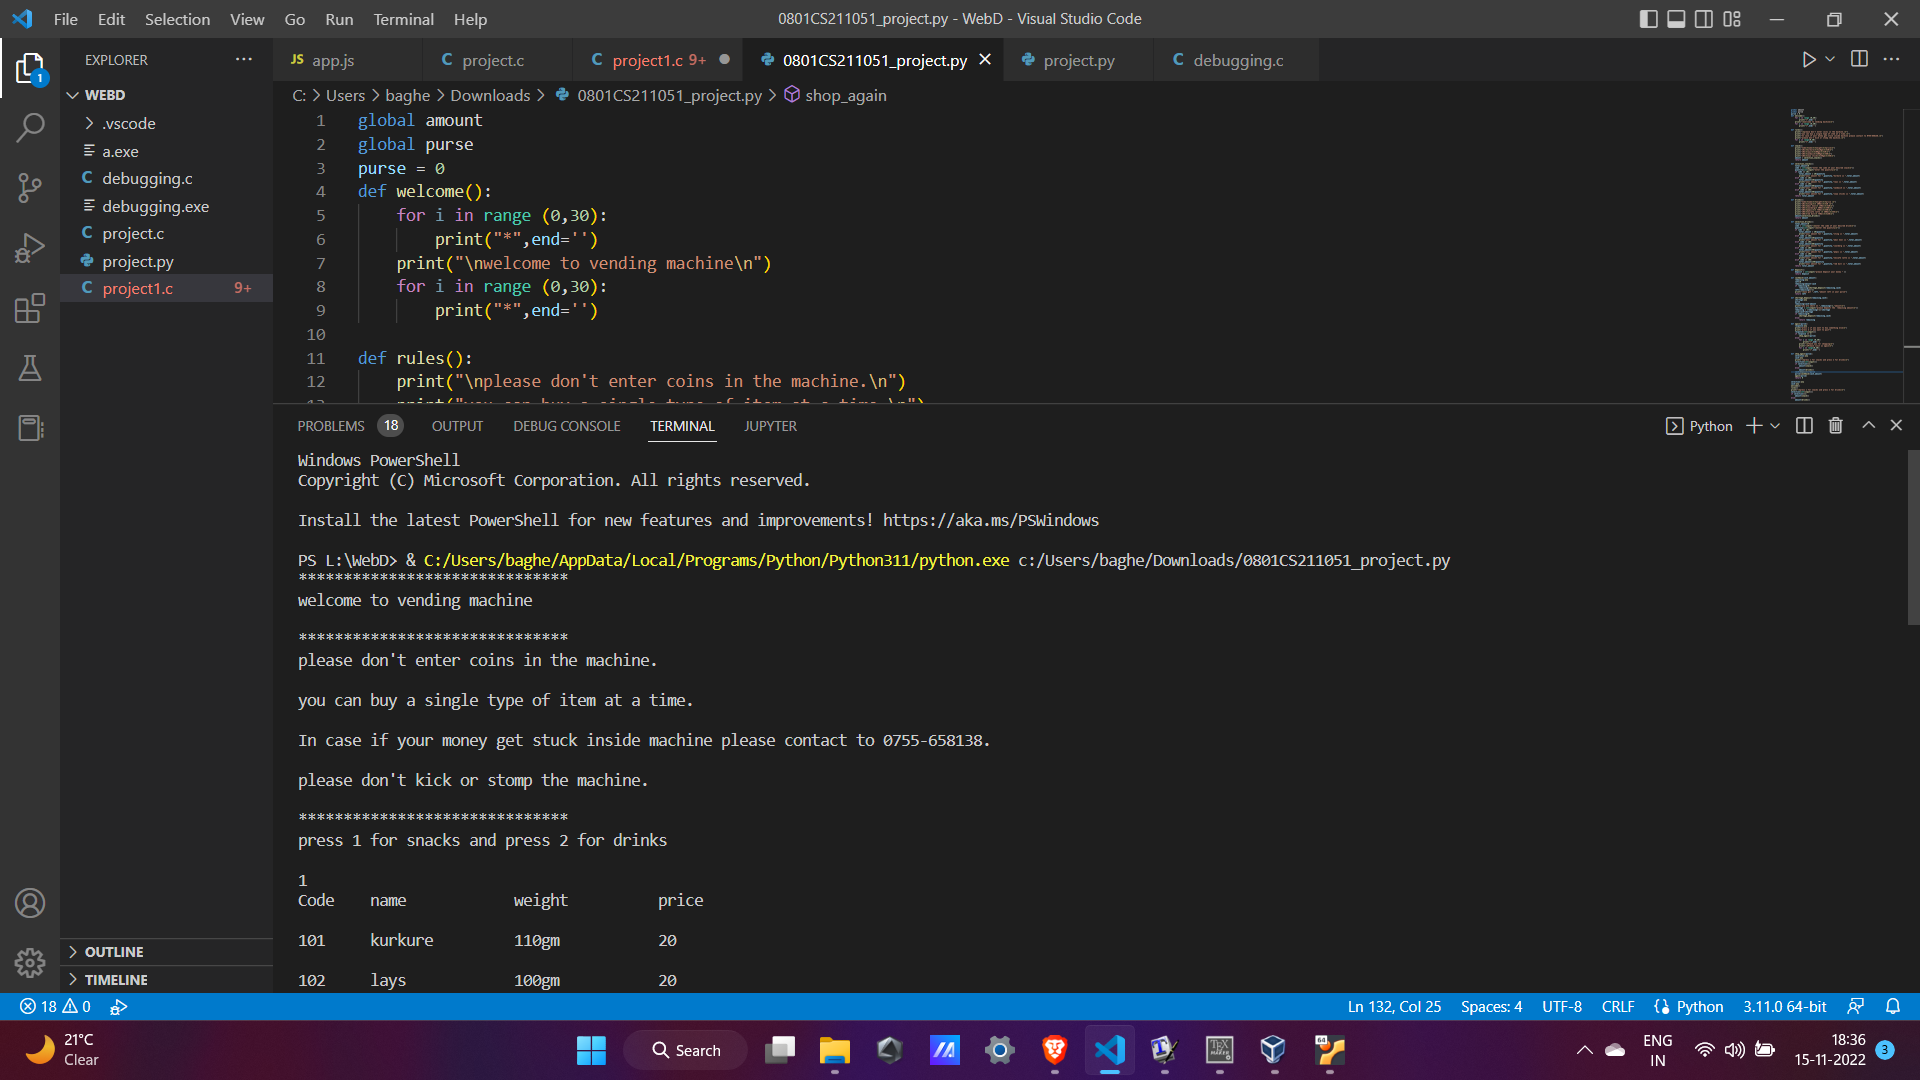
\includegraphics[scale=0.3]{python output1}\\
\bigskip
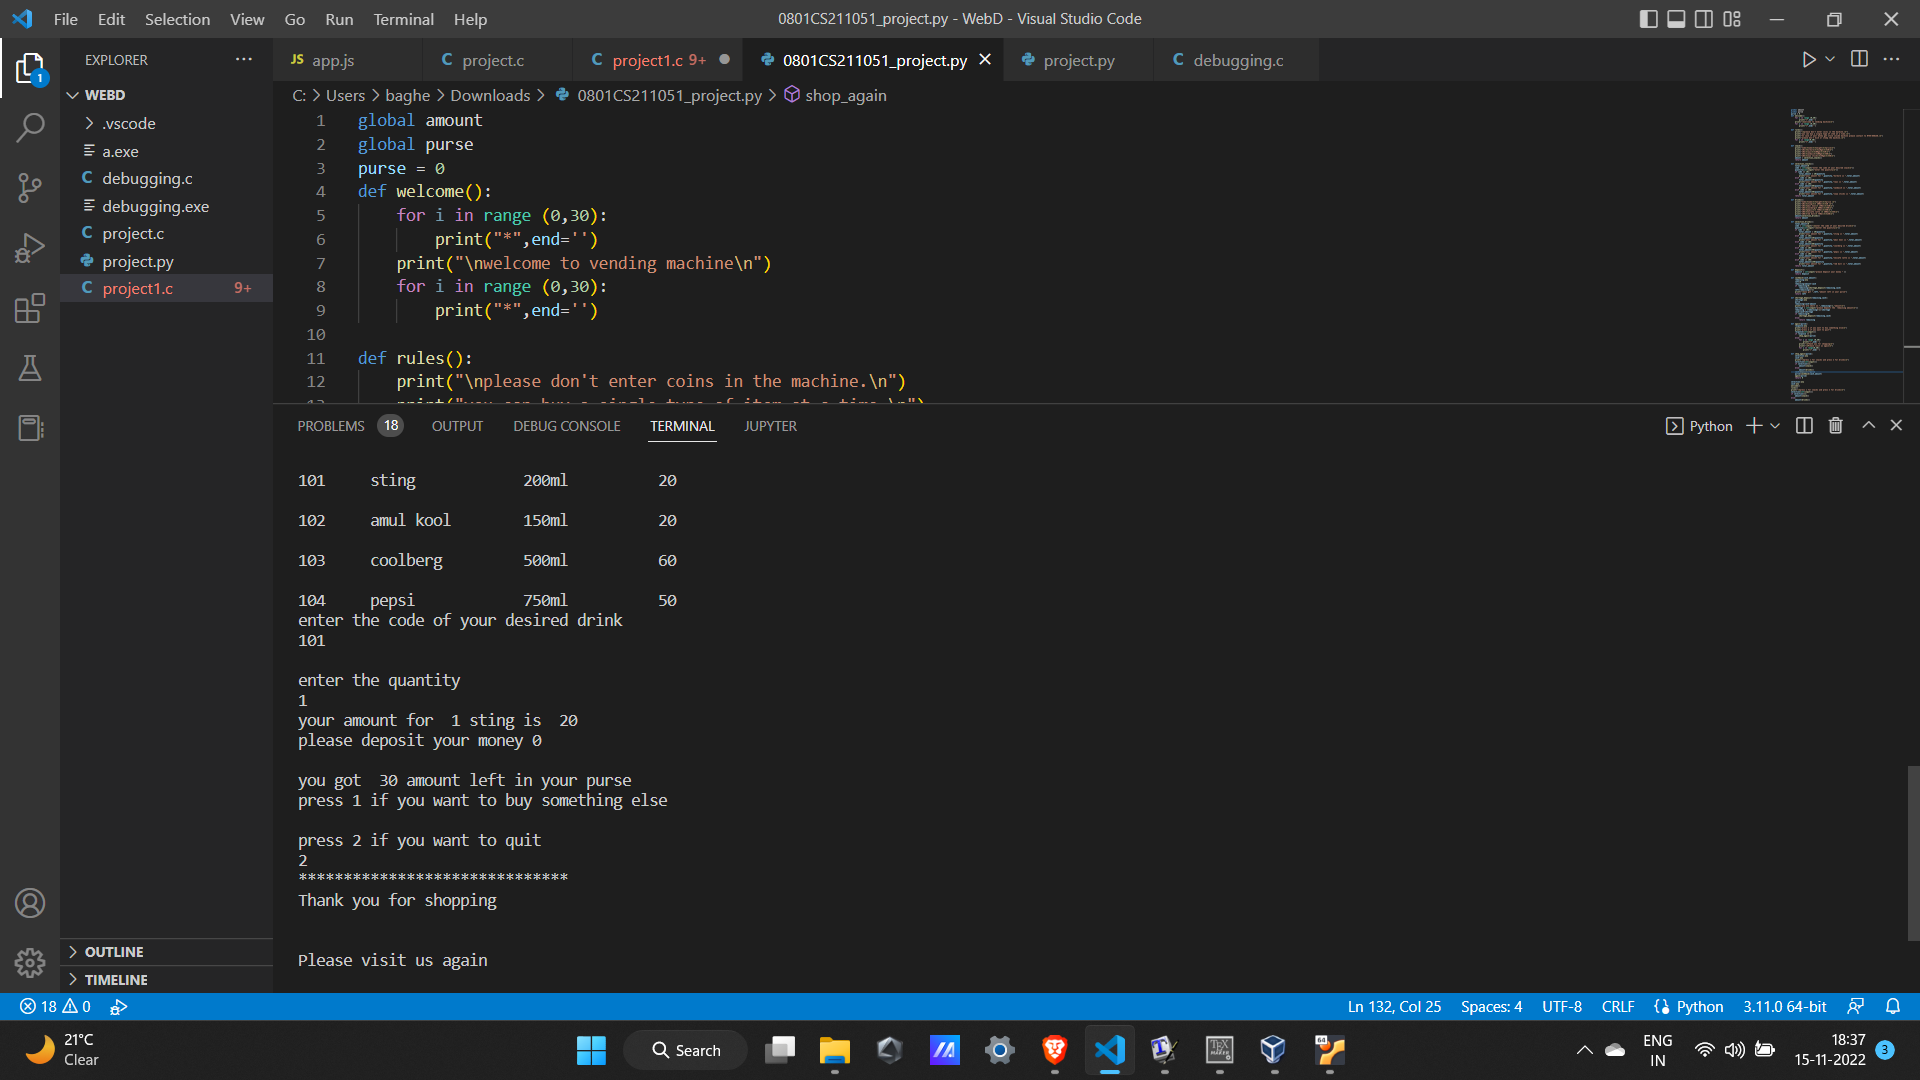
\includegraphics[scale=0.3]{python output2}
\end{center}
\end{flushleft}
\end{document}